%\chapter[<ToC-title>]{<Title>} 
\chapter[\AreaAggToCTitle]{\AreaAggTitle} 
\label{chap:AreaAgg}
%appear at the top of the pages
\chaptermark{\AreaAggChapterMark}

The land-cover area is of significant importance on maps.
When users zoom out, some land-cover areas become
too tiny to be seen, which result in visual clutter.
In order to provide users 
with good visual experience during zooming operations,
we propose to remove these tiny areas.
We plan to achieve this goal by 
aggregating them into neighboring land-cover areas.
A \emph{land-cover map} is a planar subdivision in which 
each area belongs to a land-cover class or \emph{type}.
Suppose that there are two land-cover maps of different scales 
that cover the same spatial region.
We consider the problem of finding a sequence 
of small incremental changes that gradually transforms 
the larger-scale map (the \emph{start map}) to 
the smaller-scale map (the \emph{goal map}).
We use this sequence to generate and show land-cover maps at 
intermediate scales (see \fig\ref{fig:AreaAgg_example}).
In this way, we try to avoid large and discrete changes
during zooming.

With the same motivation, 
a strategy of hierarchical schemes has been proposed.
This strategy generalizes a more-detailed representation 
to obtain a less-detailed representation 
based on small incremental changes, 
e.g., the Generalized Area Partitioning tree (GAP-tree).
This tree can be constructed if only the larger-scale map is given
\citep{vanOosterom2005} 
or if both the larger-scale map and the smaller-scale map 
are given \citep{HaunertDilo2009}.
Typically, the next change in such a sequence 
is determined locally, in a greedy fashion.  
If we insist on finding a sequence that is optimal 
according to some global measure,
the problem becomes complicated.

\begin{figure}[tb]
\centering
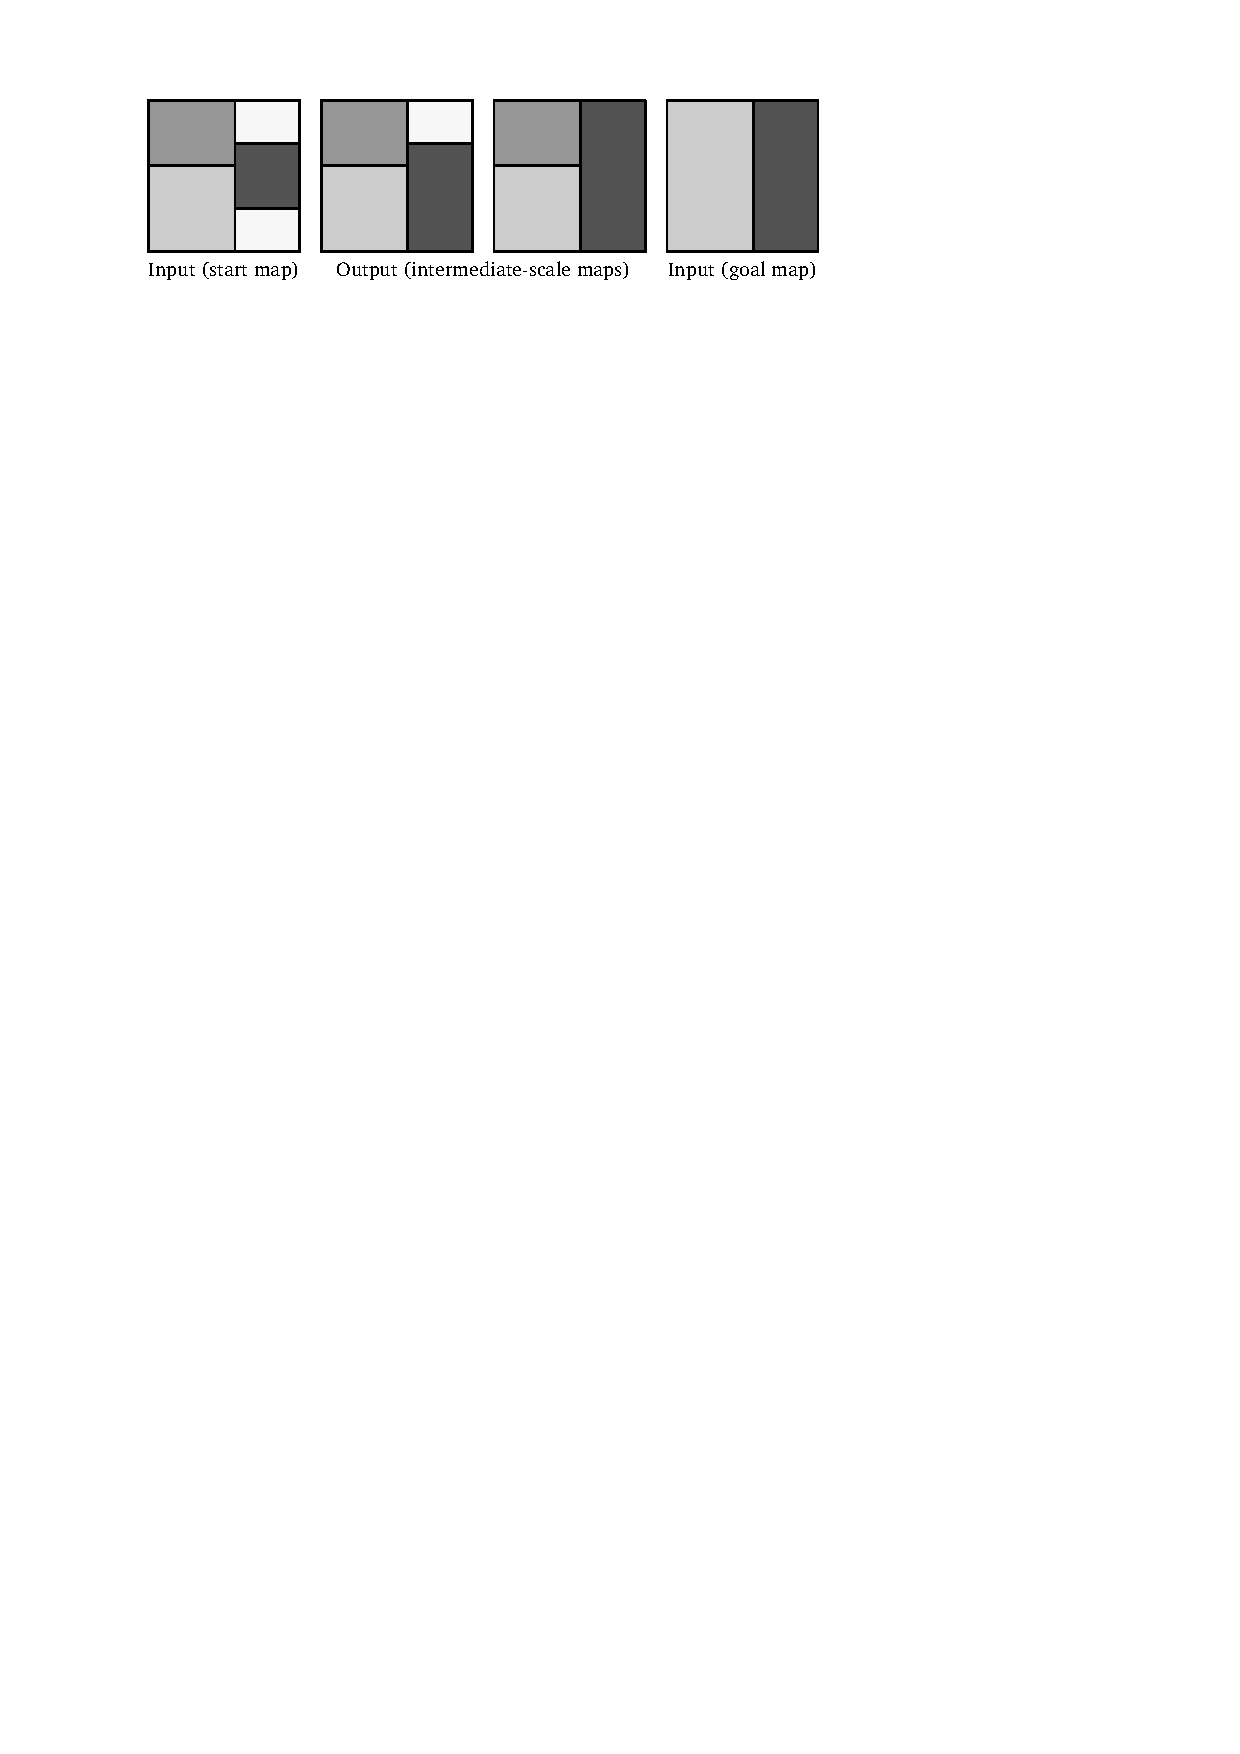
\includegraphics[page=1]{AreaAgg_Preliminaries}
\caption{The input and a possible output for an instance of 
our problem.}
\label{fig:AreaAgg_example}
\end{figure}

We assume that there exist many-to-one relationships 
between the areas of the start map and the areas of the goal map.
This assumption is based on the fact that many algorithms 
\parencite[e.g.,][]{HaunertWolff2010AreaAgg,
vanSmaalen2003,Oehrlein2017Aggregation}
result in many-to-one relationships
when aggregating land-cover areas.
Their inputs and generalized results together
can be used as our inputs.
However, we should not use those algorithms
to generate a sequence of maps at different scales
because those algorithms do not take into account 
the consistence between the generated maps.
We use both a start map and a goal map instead of using only the start map
because our generated maps at intermediate scales should be able to
benefit from a goal map with high quality.
We term the areas of the goal map \emph{regions}.
That is, every region is the union of a set of areas 
on the start map.
The type of a region may differ from the types of its 
components. 
For example, a small water area together with 
multiple adjacent forest areas may constitute 
a large forest region on the smaller-scale map.
However, we assume that every region, on the goal map, 
contains at least one area of the same type on the start map.
Our assumptions hold if the goal map has been produced 
with an automatic method for area aggregation, 
for example, by the method of \citet{HaunertWolff2010AreaAgg}.
That method produces a land-cover map at a single smaller scale, 
given a land-cover map at a larger scale.
Although \textcite{HaunertWolff2010AreaAgg}
attain results of high quality, 
they do not produce a sequence of land-cover maps.

Our method can also be extended to find an aggregation sequence 
for two maps (a start map and a goal map) that are from different sources.
In that case, one could compute a map overlay of the two maps
and use the result 
(with combined boundaries from both input maps and land cover classes 
from the given large-scale map) 
as the start map.

In this chapter, we try to find an optimal sequence
to aggregate the land-cover areas on the start map
one by one until we arrive at the goal map.
We first independently deal with each region of the goal map 
(with its components on the start map).
Once we have found an aggregation sequence for each region, 
we integrate all the sequences into an overall sequence,
which transforms the start map into the goal map
(see \fig\ref{fig:AreaAgg_IntegrateSequence}). 
Our aggregation sequence may be cooperated with
the GAP-face tree \citep{vanOosterom2005},
the map cube model \citep{Timpf1998},
or ScaleMaster \citep{Brewer2007Guidelines,Touya2013ScaleMaster}, 
to support on-the-fly visualization.
Smoothly (dis-)appearing areas can be realized
by integrating our results into the \emph{space-scale cube}
\parencite{vanOosterom2014tGAP,vanOosterom2014tGAPSSC}.

\begin{figure*}[tb]
\centering
\includegraphics[page=2]{AreaAgg_Preliminaries}
\caption{Integrating two aggregation sequences 
	of different regions: 
	the resulting sequence contains the given sequences 
	as subsequences and 
	always takes the subdivision with smallest patch next.
	The gray arrows show the integration of the two regions.
}
\label{fig:AreaAgg_IntegrateSequence}
\end{figure*}

\mypar{Contribution}
We formally model our problem, 
analyze the size of our model in a worst-case scenario,
introduce our methods,
and present the basic concepts of our method
(\sect\ref{sec:AreaAgg_Preliminaries}).
We define our cost functions 
(\sect\ref{sec:AreaAgg_CostFunctions}).
We prove that our problem is NP-hard
(\sect\ref{sec:AreaAgg_NP-hardness}).
Then, we develop and compare three methods 
for finding aggregation sequences.
First, we present 
a greedy algorithm (\sect\ref{sec:AreaAgg_Greedy}).
Second, we develop a new global optimization approach
based on the \Astar algorithm 
(\sect\ref{sec:AreaAgg_AStar}).
Third, we model our pathfinding problem as
an \emph{integer linear program} (ILP), 
and we solve this ILP with minimizing our cost function
(\sect\ref{sec:AreaAgg_ILP}).
Our ILP uses binary (0--1) variables. 
These variables help us to model our problem, 
but in general, it is NP-hard 
to solve an ILP optimally.
By comparing with the greedy algorithm, 
which is used as a benchmark,
we are able to see whether \Astar or the ILP-based algorithm, 
which are more complex and slower, indeed perform better.  
Our case study 
uses a dataset of the German topographic database ATKIS 
(\sect\ref{sec:AreaAgg_CaseStudy}).
In the concluding remarks, we show possible ways to improve our 
methods (\sect\ref{sec:AreaAgg_Conclusions}). 

We do not deal with simplifying polylines in this chapter.
The simplification can be handled separately from the
aggregation of areas, for example, 
by using one method of 
\textcite{Douglas1973},
\textcite{Saalfeld1999},
or \textcite{Wu2004DP}.
Those methods can be used to set up 
the binary line generalisation tree (BLG-tree) of
\textcite{vanOosterom1995Development},
which is a hierarchical data structure that 
defines a gradual line simplification process.
%
Although splitting polygons is a good step
of generalizing land-cover areas,
we do not integrate it into our method at this moment.
Some examples of splitting are as follows.
\textcite{Smith2007MasterMap,Thiemann2018LandCover} 
proposed to split tiny polygons 
and then to merge the split parts into the neighboring polygons.
\textcite{Meijers2016Split} developed an algorithm 
to split a polygon (the splittee) 
based on a constrained Delaunay triangulation.
During splitting, their algorithm is capable of
taking into account
the attractivenesses between the splittee and its neighbors.
When merging, a more attractive neighbor 
will get a larger portion from the splittee.


\section{Preliminaries}
\label{sec:AreaAgg_Preliminaries}

We show how to compute an aggregation sequence 
for a single region, $R$. 
For a goal map with many regions,
we ``interleave'' the sequences for each of them
with respect to the order of the smallest patches 
(see for example \fig\ref{fig:AreaAgg_IntegrateSequence}).
This integration is similar to the merge step in the 
Mergesort algorithm; 
see \textcite[\sect2.3]{Cormen2009}.
To allow us to describe our method more easily,
below we assume that the goal map has only one region.
This region consists of~$n$ land-cover 
areas (components) on the start map. 
In other words, the union of the~$n$ land-cover areas 
is the only region on the goal map.



To find a sequence of small changes 
that transforms the start map into the goal map,
we require that 
every change involves only two areas of the current map.
More precisely, in each step the smallest area~$u$ is merged 
with one of its neighbors~$v$ 
($v$ does not have to be the smallest neighbor)
such that~$u$ and~$v$ are replaced by their union.
The type of the union is restricted to be 
the type of either~$u$ or~$v$.
If the union uses the type of~$u$, 
we say that area~$v$ is \emph{aggregated into} area~$u$, 
and vice versa. 
How to aggregate exactly is decided by 
optimizing a global cost function
(see \sect\ref{sec:AreaAgg_CostFunctions}).
This requirement ensures that the 
size of the smallest area on the map increases in each step.
Hence, the sequence reflects a gradual reduction of the 
map's scale.
From another perspective, 
we consider the smallest area as the least important, 
rather than involving more rules for (non-)importance. 
Even though the requirement reduces 
the number of possible solutions,
there is still enough room for optimization 
since we leave open with
which of its neighbors the smallest area is aggregated.
We term a sequence of changes 
that adheres to our smallest-first requirement simply 
an \emph{aggregation sequence}.


\subsection{Model}
\label{sec:AreaAgg_Model}
We consider a directed graph $G_\mathrm{S}$, 
which we call the \emph{subdivision graph} 
(see \fig\ref{fig:AreaAgg_SubdivisionName}). 
The node set $V_\mathrm{S}$ of~$G_\mathrm{S}$ 
contains nodes for all the
possible maps (or \emph{subdivisions}), including the start map, 
all possible intermediate-scale maps, and the goal map.
The arc set~$E_\mathrm{S}$ of~$G_\mathrm{S}$ 
contains an arc $(\Pnode, P_{t+1,j})$ 
between any two maps~$\Pnode$ and~$P_{t+1,j}$ in~$V_\mathrm{S}$ 
if~$P_{t+1,j}$ can be reached from~$\Pnode$ 
with a single aggregation operation,
involving a smallest area.
On this basis, any directed path in~$G_\mathrm{S}$ 
from the start map to the goal map
defines a possible aggregation sequence.

\begin{figure}[tb]
\centering
\includegraphics[page=3]{AreaAgg_Preliminaries}
\caption{The subdivision graph, $G_\mathrm{S}$. 
	The nodes of the graph are the subdivisions. 
	There is an arc	from subdivision~\Pnode 
	to subdivision~${P}_{t+1,j}$ 
	if~${P}_{t+1,j}$ is the result of 
	an aggregation step from~\Pnode.}
\label{fig:AreaAgg_SubdivisionName}
\end{figure}


\subsection{Notation}
\label{sec:AreaAgg_Notation}

We represent each land-cover area by a polygon with a type.
We denote by~$P$ the set of polygons on the start map.
We use~$p$, $q$, $r$, or~$o$ to denote polygons.
A \emph{patch} is a set of polygons whose union is connected. 
Each patch also has a unique land-cover type.
We use~$u$ or~$v$ to denote the patches.

Recall that we are dealing with a single region and 
there are~$n$ land-cover areas on the start map in this region. 
Hence, the desired aggregation sequence consists of~$n-1$ steps. 
There are~$n$ subdivisions on a path 
from the start map to the goal map. 
We use~$t \in T =\{1,2,\dots,n\}$ to denote \emph{time}. 
When~$t=1$, the subdivision consists of~$n$ patches, 
and there is only one patch remaining when~$t=n$.
The subdivision graph consists of layers~${L}_1,\dots,{L}_n$, 
where layer~${L}_t=\{{P}_{t,1},\dots,{P}_{t,n_t}\}$
contains every possible subdivision~\Pnode\ with~$n-t+1$ patches 
(see \fig\ref{fig:AreaAgg_ExponentialSize}).


\begin{figure}[tb]
\centering
\includegraphics[page=4]{AreaAgg_Preliminaries}
\caption{An example to show that 
    the size of subdivision graph~$G_\mathrm{S}$
	has exponential lower bound.}
\label{fig:AreaAgg_ExponentialSize}
\end{figure}

Sometimes, we need a graph to represent the adjacencies of
the land-cover areas in a subdivision,
we call such a graph $G_\mathrm{A}$
(see \fig\ref{fig:AreaAgg_Variables_Graph}). 


\begin{figure}[tb]
\centering
\includegraphics[page=3]{AreaAgg_ILP}
\caption{The graph of a subdivision.
	Each polygon of the subdivision is represented as a node 
	in the graph.
	There is an edge between two nodes
	if the corresponding two polygons are adjacent.
}
\label{fig:AreaAgg_Variables_Graph}
\end{figure} 





\subsection{Exponential Lower Bound}
\label{sec:AreaAgg_Exponential}
We now analyze the size of subdivision graph~$G_\mathrm{S}$.
Our analysis is inspired by \textcite{Keane1975Size},
where we use a row of~$n$ land-cover areas.
In our instance
(see \fig\ref{fig:AreaAgg_ExponentialSize}), 
the start map consists of~$n=2k+1$ rectangular patches,
and the goal map is simply the union of the~$n$ patches.
The patches have area 
sizes~$
%\left( 
100 + \frac{1}{n}, 99+ \frac{2}{n}, 
100 + \frac{3}{n}, 99+ \frac{4}{n}, \ldots, 
99 + \frac{n-1}{n}, \text{and~} 101 
%\right)
$, 
from left to right.
According to our rule, we always 
aggregate the smallest patch with one of its neighbors.
Therefore, in the first~$k$ steps from the start map,
we aggregate every other patch with one of its neighbors.
However, we do not know which one is the right choice
at each of the steps
in order to minimize our costs (see \sect\ref{sec:AreaAgg_CostFunctions}).
We have to try both of the two choices,
aggregating with the left patch or with the right one.
As a result, there are~$2^k = 2^{(n-1)/2}$ subdivisions 
in layer~$L_{k+1}$.
That is to say, the size of subdivision graph~$G_\mathrm{S}$
has exponential lower bound.


\subsection{Methods}
\label{sec:AreaAgg_Methods}

Our idea is to obtain an optimal aggregation sequence through 
computing a path with minimum weight, from the start to the goal 
(see \fig\ref{fig:AreaAgg_SubdivisionName}).
This idea obviously requires that the arc weights are 
set such that a minimum-weight start--goal
path does actually correspond to an aggregation sequence of 
maximum cartographic quality.  
Moreover, putting the idea to practice is far from trivial 
since graph~$G_\mathrm{S}$ can be huge.
We compare a greedy algorithm, \Astar, and an ILP-based algorithm
in finding such paths.
Note that our inputs are only
subdivisions~$\Pstart$ and~$\Pgoal$
(see \fig\ref{fig:AreaAgg_SubdivisionName}).
We generate a subdivision (node) only when we want to visit it.

In directed acyclic graphs, shortest paths can be found slightly faster 
than in general directed or undirected graphs.
An off-the-shelf shortest-path algorithm for directed acyclic graphs
%\parencite[e.g.,][\sect25.2]{Cormen2009},
(e.g., \textcite[\sect25.2]{Cormen2009}),
however, will explore the whole graph, which has exponential size.
The \Astar algorithm can be seen as 
a refinement of Dijkstra's algorithm, 
which for a user-specified given source 
computes shortest paths to all other nodes in an edge-weighted graph
\parencite{Dijkstra1959}. 
Even when using Dijkstra's algorithm 
to compute only a single shortest path to a user-specified destination, 
a large number of nodes need to be explored. 
The same holds for shortest-path algorithms 
that make use of a topological order of the nodes 
in a directed acyclic graph. 
Compared to these algorithms, 
the \Astar algorithm can greatly reduce the number of explored nodes.
The challenge in our work was to tune the A* algorithm such that it
explores only a small fraction of the graph.





\section{Cost Functions}
\label{sec:AreaAgg_CostFunctions}

\fig\ref{fig:AreaAgg_SubdivisionName} shows that there are many 
ways to aggregate from the start map to the goal map.
Apparently, some of the ways are more reasonable than others.
In our example, we consider 
sequence~$(P_{1,1}, P_{2,1},P_{3,1},P_{4,1})$ 
more reasonable than 
sequence~$(P_{1,1}, P_{2,4},P_{3,5},P_{4,1})$.
This is because that the dark area should not expand so much
when the target color is light gray.
We want to provide users with a most reasonable sequence 
because we believe that an unreasonable sequence irritates users.
To find a most reasonable sequence, we introduce cost functions.
In the cost functions, we charge a higher penalty 
when an aggregation step is less reasonable.
As a result, by minimizing the overall cost of an aggregation 
sequence, we find a most reasonable sequence.

It is difficult to define what \emph{reasonable} exactly means 
because users may have different preferences.
Four preferences have been discussed by
\textcite{Cheng2006}; see \fig\ref{fig:AreaAgg_Preferences}.
A small land-cover area can be aggregated into another area 
that isolates the area 
(\fig\ref{fig:AreaAgg_Preferences}b), 
that is the largest neighbor 
(\fig\ref{fig:AreaAgg_Preferences}c), 
that shares the longest boundary 
(\fig\ref{fig:AreaAgg_Preferences}d), or 
that has the most similar type
(\fig\ref{fig:AreaAgg_Preferences}e).
To keep our aggregation problem independent of user preferences,
our cost function takes two aspects into account: 
one based on semantics and 
the other based on shape.
%
In terms of semantics, we require that 
the \emph{type} of a land-cover area changes 
as little as possible.
This requirement means that we prefer, for example, 
aggregating an area with type \emph{swamp} 
into an area with type \emph{wet ground} 
rather than into an area with type \emph{city}.
%
In terms of shape, we hope to have areas 
which are as \emph{compact} as possible.
Our argument is that an area is easier 
to be identified by a human being 
if it is more compact (less clutter).
%
We also consider the total \emph{length} 
of the interior boundaries as an alternative compactness;
we consider subdivision~\Pnode 
as more compact than subdivision~$P_{t,i'}$ 
if the total length of the interior boundaries of~\Pnode 
is less than that of~$P_{t,i'}$.
We add this alternative because we want to make a comparison 
involving an ILP, 
where a \emph{linear} cost function must be used.
Note that most compactness measures
are \emph{not} linear;
for example, see \textcite{Maceachren1985,Li2013Compactness}.
Although the length of interior boundaries 
is not sufficiently precise 
to describe compactness \parencite{Young1988},
it is often used as a fair alternative
when compactness is considered in an ILP
\parencite[e.g.,][]{Minas2016,Wright1983}.
\textcite{HaunertWolff2010AreaAgg} employed 
the centroids of a set of land-cover areas.
One of their costs is the sum of the distances 
from the centroids to a \emph{reference point}.
The reference point is one of the centroids
that minimizes the sum.
The sum of the distances can be computed linearly.
We use the length of interior boundaries 
instead of the distance of centroids because the former 
is more relevant to the shapes of the patches.
Also, \textcite{Harrie2015Readability} showed that
longer lines generally yield lower map readability.

\begin{figure}[tb]
\centering
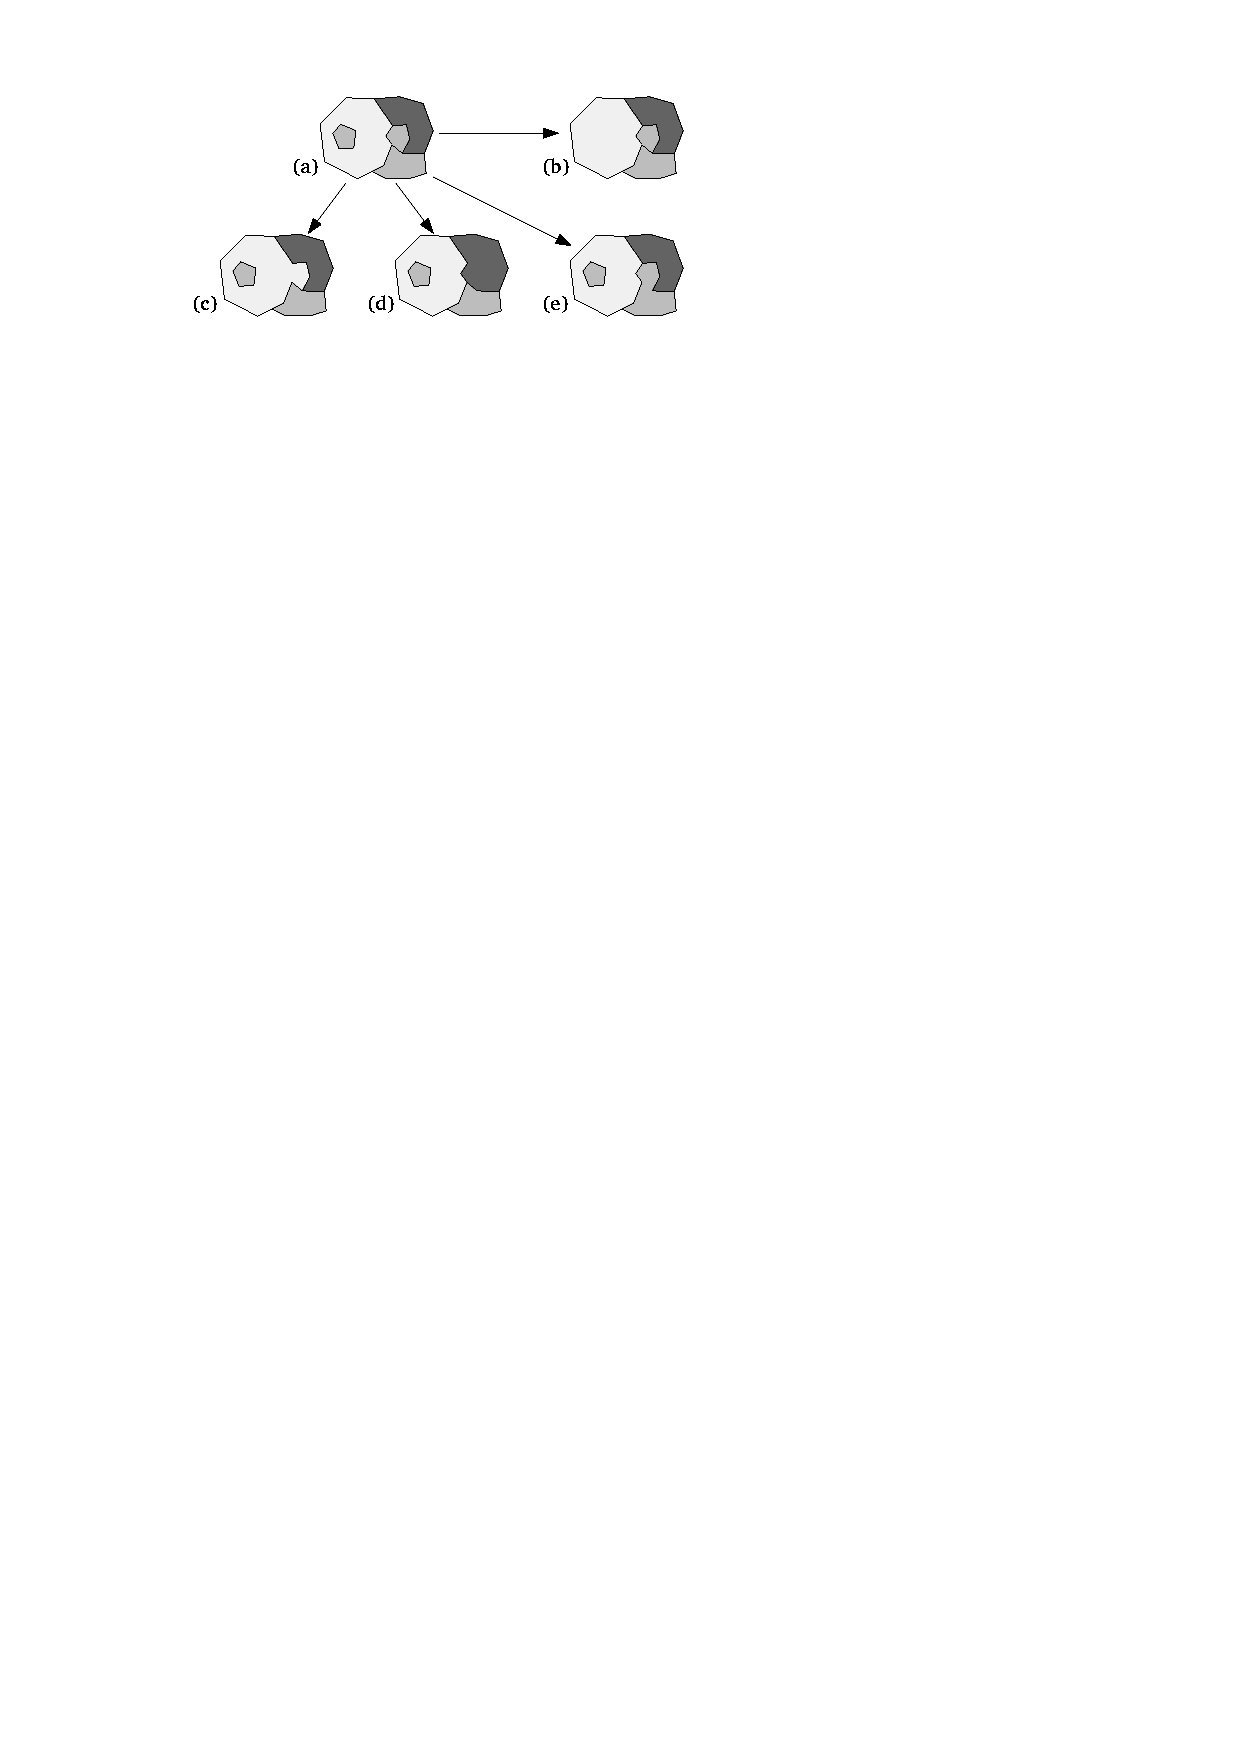
\includegraphics[page=1]{AreaAgg_CostsAndEstimations}
\caption{Aggregating land-cover areas 
	according to different preferences
    by \textcite{Cheng2006}.
	Aggregating a small land-cover area into another one 
	that isolates the area (b), 
	that is the largest neighbor (c), 
	that shares the longest boundary (d), or 
	that has the most similar type (e).}
\label{fig:AreaAgg_Preferences}	
\end{figure}


\subsection{Cost of Type Change}
\label{sec:AreaAgg_f_type}

Suppose that we are at the step of aggregating 
from subdivision~$P_{s,i}$ to subdivision~$P_{s+1,j}$. 
In this step, patch~$u$ is aggregated into patch~$v$
(see \figs\ref{fig:AreaAgg_FirstStep}a 
and \ref{fig:AreaAgg_FirstStep}b).
We denote the types of the two patches by~$T(u)$ and~$T(v)$. 
We define the cost of type change of this step by
\begin{equation}
\label{eq:f_type}
f_\mathrm{type}(P_{s,i},P_{s+1,j})=\frac{A_{u}}{A_R}
\cdot
\frac{d_\mathrm{type}(T(u),T(v))}{d_\mathrm{type\_max}},
\end{equation}
where~$A_u$ is the area of patch~$u$, 
and~$A_R$ is the area of region~$R$
(see \sect\ref{sec:AreaAgg_Preliminaries}).
We use~$A_R$ and~$d_\mathrm{type\_max}$ 
to normalize the cost of type change. 
Constant~$d_\mathrm{type\_max}$, the maximum cost over all type changes,  
is known from the input. 
The input specifies
cost~$d_\mathrm{type}(T_1,T_2)$ of changing type~$T_1$ to type~$T_2$.
Specifically, we denote by~$T_\mathrm{goal}$ the type of 
the patch on the goal map.
For simplicity, we use a metric 
as the cost function of type change
(see \sect\ref{sec:AreaAgg_CaseStudy}).
A metric distance is symmetric, 
which is different from the asymmetric one used in
\textcite{Dilo2009tGAP}.
In their definition, for example, 
the distance from type \emph{building} to type \emph{road} is~$0.5$,
but the distance from \emph{road} to \emph{building} is~$0$.

For path $\Pistar=(P_{1,i_1}, P_{2,i_2}, \dots, 
P_{\tstar,i_{\tstar}})$,
we define the cost of type change %over the steps 
by
\begin{equation}
\label{eq:g_type}
g_\mathrm{type}(\Pistar)=
\sum_{s=1}^{t-1}f_\mathrm{type}(P_{s,i_s},P_{s+1,i_{s+1}}).
\end{equation}

\begin{figure}[tb]
\centering
\includegraphics[page=2]{AreaAgg_CostsAndEstimations}
\caption{An aggregation step, 
	where patch~$u$, the dark patch at the top,
	is aggregated into patch~$v$.
	\figs(c) and~(d) respectively show the number of 
	edges and the lengths of the interior polylines after 
	the aggregation.}
\label{fig:AreaAgg_FirstStep}	
\end{figure}

\subsection{Cost of Compactness}
\label{sec:AreaAgg_f_comp}

We use the compactness definition of \citet{Frolov1975}, 
i.e., the compactness value of a patch, say,~$u$ is
\begin{equation}
\label{eq:comp}
c(u)=\frac{2 \sqrt{\pi A_u}}{l_u},
\end{equation}
where~$A_u$ and~$l_u$ are 
the area and the perimeter. 
For subdivision \Psnode, we denote by~$C(\Psnode)$ 
the set of the patches' compactness values.

We wish to maximize the sum of the average compactness values 
over all intermediate maps,
while our objective will be
minimizing a cost function.
To adapt the average compactness to our methods, 
we define and minimize a cost related to compactness.
Recalling that there are~$n-s+1$ patches at time~$s$,
we define the cost of compactness for subdivision~\Psnode as
\begin{equation}
\label{eq:f_comp}
f_\mathrm{comp}(\Psnode)=
\frac{1-\frac{1}{n-s+1} \sum_{c\in C(\Psnode)}c}{n-2},
\end{equation}
where we use values~$n-s+1$ and~$n-2$ to normalize 
the cost of compactness.

For path $\Pistar$ (see \sect\ref{sec:AreaAgg_f_type}),  
we define the cost of compactness over all 
intermediate maps
(that is, neglecting~$P_{1,1}$ 
and the last subdivision in the path) by
\begin{equation}
\label{eq:g_comp}
g_\mathrm{comp}(\Pistar)=
\sum_{s=2}^{\tstar-1}f_{\mathrm{comp}}(P_{s,i_s}).
\end{equation}


\subsection{Cost of Length}
\label{sec:AreaAgg_costlength}

We denote the set of interior boundaries 
for a subdivision~$\Psnode$ by~$B(\Psnode)$.
The cost in terms of interior length of 
this subdivision is defined as
\begin{equation}
\label{eq:f_length}
f_\mathrm{lgth}(\Psnode)=
\frac{\big(\sum_{b\in B (\Psnode)} 
	|b|\big)\big/D(s)}{n-2}, 
\end{equation} 
where 
\begin{equation}
\label{eq:AreaAgg_Norm}
D(s)=\frac{n-s}{n-1} \sum_{b\in B (\Pstart)} |b|.
\end{equation}
Function~$D(s)$ computes the ``expected'' total length of 
the interior boundaries at time~$s$,
where we expect that this total length decreases linearly
according to time~$s$.
In special,~$D(1) = \sum_{b\in B (\Pstart)} |b|$
and~$D(n) = 0$.
Similarly to \eq\ref{eq:f_comp}, 
we use~$D(s)$ and~$n-2$ to normalize 
the cost of length.


For path~$\Pistar$ (see \sect\ref{sec:AreaAgg_f_type}), 
we define the cost of length over all 
intermediate maps 
(that is, neglecting~$P_{1,1}$ 
and the last subdivision in the path) by
\begin{equation}
\label{eq:g_length}
g_\mathrm{lgth}(\Pistar)=
\sum_{s=2}^{\tstar-1}f_{\mathrm{lgth}}(P_{s,i_s}).
\end{equation}

Note that in theory, a patch, $u$, with a small perimeter 
can be extremely non-compact 
according to measure~$c(u)$ in \eq\ref{eq:comp}, 
thus the two measures, $f_\mathrm{comp}$ and~$f_\mathrm{lgth}$, 
are not interchangeable. 
However, if we assume that all areas of the map have the same size 
(i.e., $A_u$ of \eq\ref{eq:comp} is a constant), 
it would make no difference whether 
we minimize an area's perimeter 
or maximize the area's compactness~$c(u)$. 
Obviously, the areas in our dataset have different sizes. 
However, since we iteratively remove the smallest area, 
the differences do not become too large. 
Therefore, measuring the overall compactness of a map 
based on the total length of 
all the interior boundaries is quite reasonable.

\subsection{Combining Cost Functions}
\label{sec:AreaAgg_Combining}
When we generate a sequence of intermediate-scale maps,
we want to change the types of the land-cover areas 
as little as possible
and want to have compact land-cover areas.
Therefore, we combine 
the cost of type change (\eq\ref{eq:g_type})
and the cost of compactness (\eq\ref{eq:g_comp}).
That is,
\begin{equation}
\label{eq:g_1}
g_1(\Pistar)= (1-\lambda)g_\mathrm{type}(\Pistar)
+\lambda g_\mathrm{comp}(\Pistar),
\end{equation}
where~$\lambda \in [0,1]$ is a parameter 
to assign importances 
of~$f_\mathrm{type}$ and~$f_\mathrm{comp}$.
We simply use~$\lambda=0.5$ in our experiments. 
We want to find a path~$\Pi$ from~$\Pstart$ to~$\Pnode$ 
that minimizes, among all such paths,~$g_1(\Pistar)$.
Slightly abusing notation, we denote the cost of
an optimal path from~${P}_{\mathrm{start}}$ to~\Pnode 
by~$g_1(\Pnode)$.
Using $g_1(\Pnode)$, we compare a greedy algorithm and \Astar
in finding optimal sequences for area aggregation.

As said before, we want to make a comparison involving
integer linear programming 
while our cost of compactness (see \eq\ref{eq:comp})
cannot be computed linearly in an integer linear program.
Therefore, we combine 
the cost of type change (\eq\ref{eq:g_type})
and the cost of length (\eq\ref{eq:g_length}),
which can be computed linearly in an integer linear program. 
That is,
\begin{equation}
\label{eq:g_2}
g_2(\Pistar)= (1-\lambda)g_\mathrm{type}(\Pistar)
+\lambda g_\mathrm{lgth}(\Pistar).
\end{equation}
We compare the greedy algorithm, \Astar, and an ILP-based 
algorithm using~$g_2$.

\section{NP-hardness Proof}
\label{sec:AreaAgg_NP-hardness}

Although we have shown that the graph of subdivisions
has an exponential size
(see \sect\ref{sec:AreaAgg_Preliminaries}),
one may develop a clever algorithm 
to find an optimal sequence efficiently.
In the following, we prove that 
finding such a sequence is indeed NP-hard.
In the proof, we neglect the cost of compactness or the cost of length.
Considering one of the two costs 
will make the computation even more difficult.


\newtheorem{thm}{Theorem}
\begin{thm}
\textsc{AreaAggregationSequence} is NP-hard 
even if we only consider the cost of type change.
\end{thm}

\begin{proof}
Our NP-hardness proof is by reduction from 
the NP-complete problem \textsc{PlanarVertexCover}, 
which is to decide, for a given 
planar graph~$G_\mathrm{A} = (V_\mathrm{A},E_\mathrm{A})$, 
whether there exists a vertex cover 
with at most a given number~$k_\mathrm{A}$ of vertices. 
For an instance of \textsc{PlanarVertexCover}
(\fig\ref{fig:AreaAgg_Reduction}a), 
we define a corresponding instance of \textsc{AreaAggregationSequence}
whose start map consists of gray, black, and white areas and 
whose goal map consists of only one large gray patch.
The adjacency graphs of the two maps are illustrated 
in \figs\ref{fig:AreaAgg_Reduction}b and~\ref{fig:AreaAgg_Reduction}c, 
where the colors of the vertices represent 
the colors of the corresponding areas.
More precisely, for each vertex of~$G_\mathrm{A}$
in \fig\ref{fig:AreaAgg_Reduction}a, 
we define a gray vertex and a black vertex, 
which we connect with an edge. 
For each edge $\{u,v\}$ of~$G_\mathrm{A}$, 
we define two white vertices and 
connect each of them both with the black vertex for $u$
and the black vertex for $v$
(\fig\ref{fig:AreaAgg_Reduction}b).

\begin{figure}[tb]
\centering
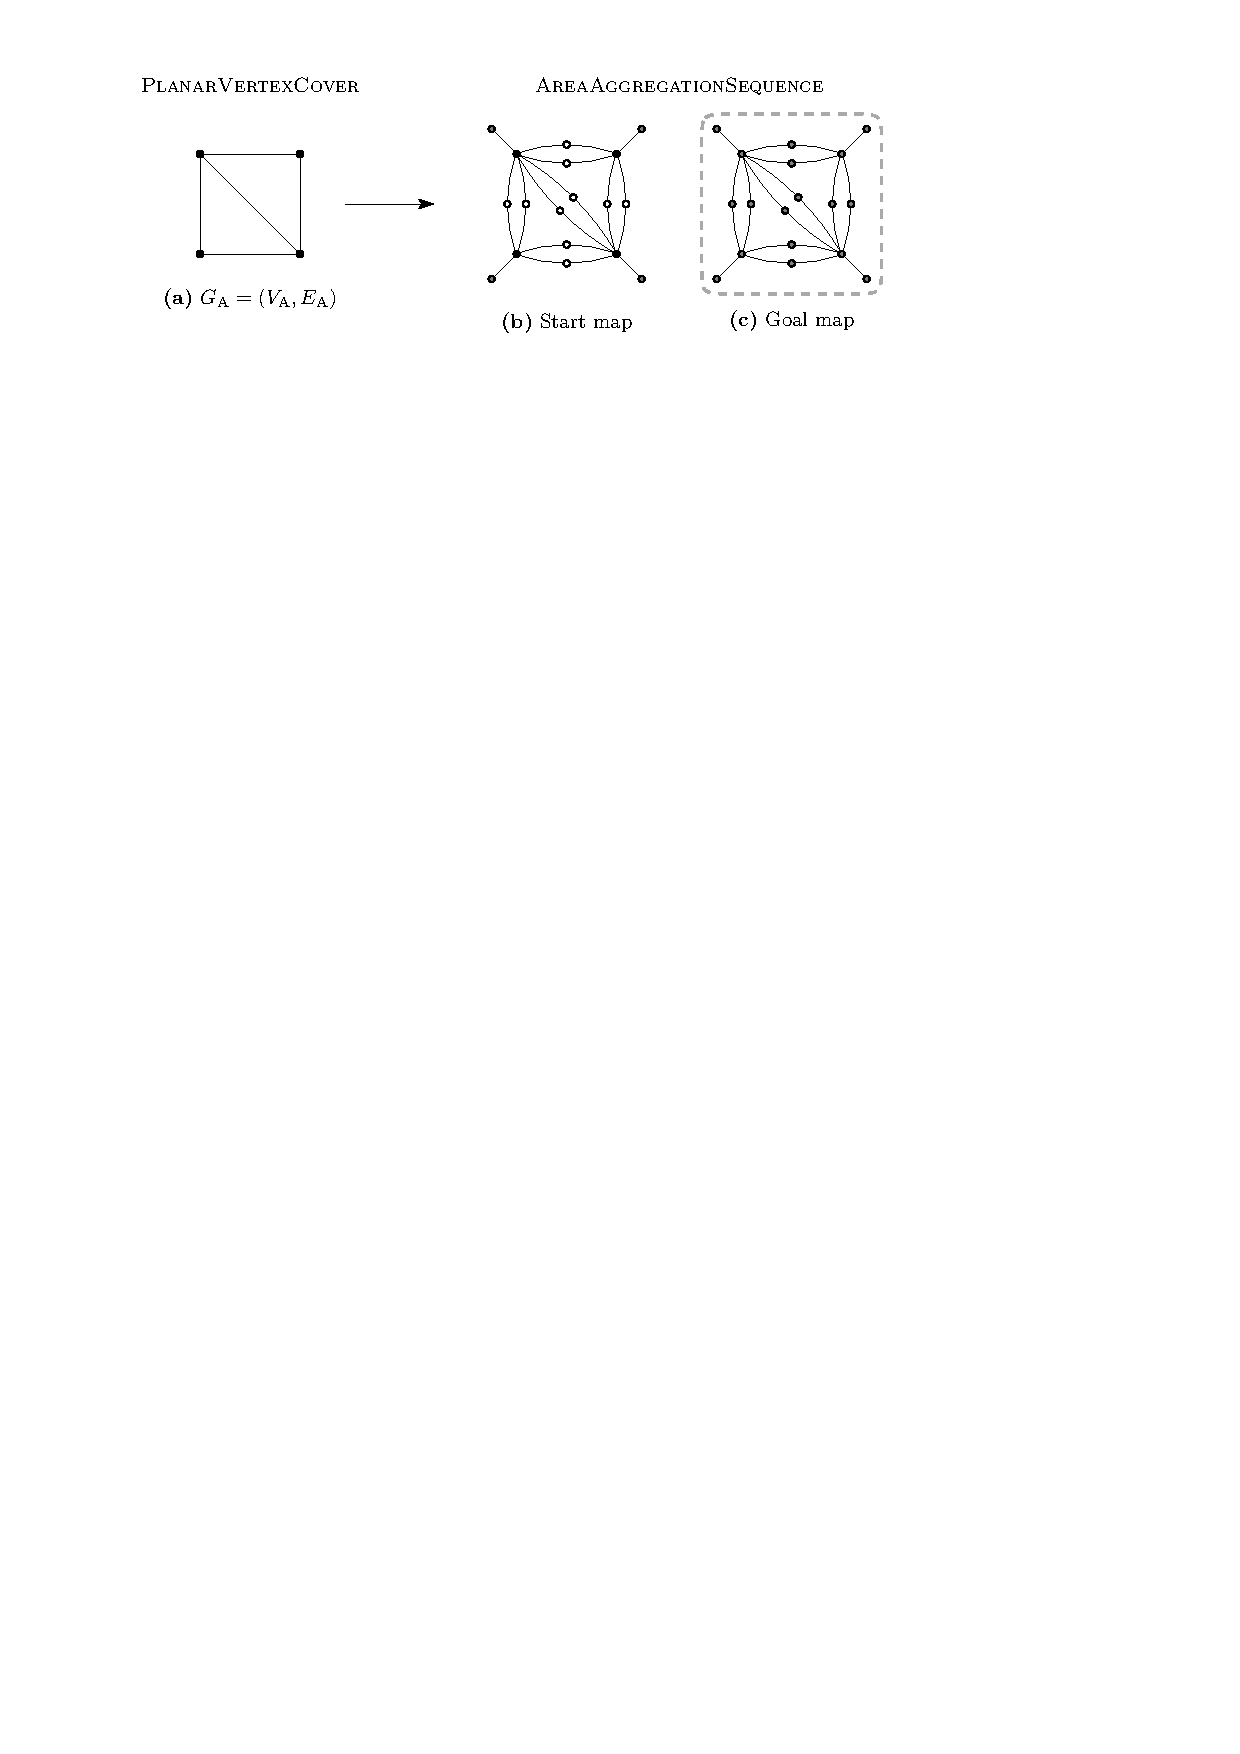
\includegraphics[page=1]{AreaAgg_NPHard}
\caption{The reduction for our NP-hardness proof.
    The dashed polygon in (c) shows 
    the merged vertices.}
\label{fig:AreaAgg_Reduction}
\end{figure}

We define the weights of the vertices 
in \fig\ref{fig:AreaAgg_Reduction}b as follows:
\begin{itemize}
\item Every white vertex has weight~$1$.
\item Every black vertex has weight~$2$.
\item Every gray vertex has weight~$2|V_\mathrm{A}| + 2|E_\mathrm{A}|$,
which is equal to the total weight of all white and black vertices.
\end{itemize}
When we merge two vertices, 
the weight of the new vertex is the sum of the two.
In each aggregation step, 
we require the smallest area to be aggregated with one of its neighbors.
The area sizes correspond to the weights of the vertices in \fig\ref{fig:AreaAgg_Reduction}b.   
Therefore, our definition of the weights to a certain degree determines 
the order in which the vertices are selected:
\begin{itemize}
\item \emph{Phase I}: In each of the first~$2|E_\mathrm{A}|$ steps, 
a white vertex is selected and merged with one of its neighbors, 
such that the white vertex receives the neighbor's color or vice versa
(\fig\ref{fig:reduction2} shows a possible result).
\item \emph{Phase II}: In each of the next~$|V_\mathrm{A}|$ steps, 
a non-gray vertex is selected and merged with one of its neighbors.
\item \emph{Phase III}: $|V_\mathrm{A}|-1$ steps remain to reach the goal map.
\end{itemize}

To complete the reduction, 
we need to define the costs of color changes. 
For any color change, 
we charge one unit of cost per unit weight.
Due to our construction, Phases II and III can be accomplished with
a total cost of~$2|V_\mathrm{A}|+2|E_\mathrm{A}|$, 
no matter how Phase I is accomplished.
This is because, after Phase I, 
every non-gray patch will be adjacent to a gray patch (vertex).
Thus, if any non-gray patch becomes selected in Phase II, 
it can be aggregated with a gray patch (vertex) and 
receive the color gray. 
This implies that Phase II costs $2|V_\mathrm{A}|+2|E_\mathrm{A}|$ 
(which is equal to the total weight of 
all initially white and black vertices) and, 
since after Phase II all patches are gray, 
Phase III does not cause any additional cost.  
It is also clear that 
there is no cheaper way to accomplish Phases II and III,
since it is impossible to color a vertex gray in Phase I.
Consequently, since the total cost of Phases II and III is fixed, 
it is only interesting to ask 
at which cost Phase I can be accomplished.
It turns out that, if $G_\mathrm{A}$ 
has a vertex cover $C_\mathrm{A} \subseteq V_\mathrm{A}$, 
then Phase I can be accomplished with cost $2|C_\mathrm{A}|$;
only the black vertices corresponding to vertices in~$C_\mathrm{A}$ 
need to change their color from black to white, and 
each of them has weight~$2$ (see \fig\ref{fig:reduction2}).
To summarize, if graph~$G_\mathrm{A}$ has a vertex cover~$C_\mathrm{A}$, 
then the corresponding instance of \textsc{AreaAggregationSequence} 
has a solution of 
total cost~$2|C_\mathrm{A}|+2|V_\mathrm{A}|+2|E_\mathrm{A}|$.

It remains to be shown that, 
if $C_\mathrm{A}^*$ is a minimum vertex cover of $G_\mathrm{A}$, 
then there is no solution with total cost 
less than $2|C_\mathrm{A}^*|+2|V_\mathrm{A}|+2|E_\mathrm{A}|$.
To see why, we assume that such a solution exists.
If we keep the black color of a vertex from $C_\mathrm{A}^*$ 
(the total cost decreases by $2$),
then we will need to at least change two white vertices
to black vertices
(the total cost increases by $2$ at least).
Therefore, we have found a contradiction to our assumption.

\begin{figure}[tb]
\centering
\includegraphics[page=2]{AreaAgg_NPHard}
\caption{The situation after Phase I has been conducted 
    such that all black vertices corresponding to a vertex cover 
    of~$G_\mathrm{A}$ have been recolored white.
    The dashed polygons show that the vertices are merged.}
\label{fig:reduction2}
\end{figure}
\end{proof}

\section{A Greedy Algorithm}
\label{sec:AreaAgg_Greedy}

A motivation for the greedy algorithm is that 
a very similar iterative algorithm has been used by
\textcite{vanOosterom2005} 
for constructing the tGAP data structure.
However, we have to make minor modifications to ensure that 
the computed aggregation sequence ends with the goal map that, 
in our situation, is given as a part of the input.
We use our greedy algorithm as a benchmark
so that we are able to see 
whether the \Astar algorithm or the ILP-based algorithm 
indeed perform better.

At any time~$t$,
our greedy algorithm aggregates the smallest patch
with one of its neighbors.
We pick the neighbor in a greedy way.
We suppose that the smallest patch,~$u$, has~$k_u$ neighbors,
then there are~$2k_u$ ways to aggregate
(when we aggregate a patch into another patch,
the union uses the type of the latter).
In order to guarantee that our final result
(e.g., the polygon of layer~$L_4$ in 
\fig\ref{fig:AreaAgg_SubdivisionName})
will have the type of~$T_\mathrm{goal}$,
we add one more rule to our greedy algorithm.
Suppose that patch~$v$ is one of~$u$'s neighbors.
The greedy algorithm aggregates~$u$ into~$v$ 
if the type distances fulfill that
$d_\mathrm{type}\left(T(u), T_\mathrm{goal}\right) 
\ge d_\mathrm{type}\left(T(v), T_\mathrm{goal}\right)$;
otherwise, the algorithm aggregates~$v$ into~$u$.
This rule excludes, say,~$k_e$ aggregation choices,
and we have~$2k_u - k_e$ choices left.
Then we compute the costs for each of 
the~$2k_u - k_e$ aggregation choices
and select the aggregation that has the least cost.
In other words, we aggregate the smallest patch with 
its most \emph{compatible} neighbor.

In accordance with our two combinatorial costs in 
\sect\ref{sec:AreaAgg_Combining},
we define two cost functions.
Suppose that we are at the step of aggregating 
from subdivision~$P_{s,i}$ to subdivision~$P_{s+1,j}$.
The first cost function is 
\begin{equation}
\label{eq:f_1}
f_1(P_{s,i},P_{s+1,j})=
(1-\lambda)f_\mathrm{type}(P_{s,i},P_{s+1,j})
+\lambda f_{\mathrm{comp}}(P_{s+1,j}).
\end{equation}
The second cost function is
\begin{equation}
\label{eq:f_2}
f_2(P_{s,i},P_{s+1,j})=
(1-\lambda)f_\mathrm{type}(P_{s,i},P_{s+1,j})
+\lambda f_{\mathrm{lgth}}(P_{s+1,j}).
\end{equation}
We take one of the~$2k_u - k_e$ aggregation choices 
according to \eqs\ref{eq:f_1} or~\ref{eq:f_2}
in our two experiments.
The cost of a whole sequence can be computed by
\eqs\ref{eq:g_1} or~\ref{eq:g_2}.







\section{Using the \texorpdfstring{\Astar Algorithm}{A* Algorithm}}
\label{sec:AreaAgg_AStar}

\sect\ref{sec:AreaAgg_Preliminaries} has shown that
the size of finding an optimal aggregation sequence 
can be exponential.
That is to say, the graph~$G_\mathrm{S}$---our search space---can 
be of exponential size.
In order to avoid computing the whole graph explicitly,
we use the \Astar algorithm \parencite{Hart1968,PatelAStar}.
To save time and memory, 
we generate a subdivision, \Pnode, only 
when we are going to visit it.
\Astar uses a clever best-first search 
to find a shortest path 
from subdivision~$\Pstart$ to subdivision~$\Pgoal$.  
For \Pnode,
\Astar considers the exact cost of a shortest path 
from~\Pstart to~\Pnode 
and estimates the cost to get from~\Pnode to~\Pgoal. 
\Astar explores the nodes earlier 
if they are estimated to be closer to the goal.
\Astar can be seen as a refinement of Dijkstra's algorithm
\parencite{Dijkstra1959}.

We define~$g(\Pnode)$ to be 
the exact cost of a shortest path from~\Pstart to~\Pnode 
and define~$h(\Pnode)$ to be the estimated cost 
to get from \Pnode to~\Pgoal. 
Then, the (estimated) total cost at node~\Pnode is
\begin{equation}
\label{eq:CostTotal}
F(\Pnode)=g(\Pnode)+h(\Pnode).
\end{equation}
We use either~$g_1$ (\eq\ref{eq:g_1}) 
or~$g_2$ (\eq\ref{eq:g_2}) for~$g(\Pnode)$;
accordingly, we use either~$h_1$ (\eq\ref{eq:h_1}) 
or~$h_2$ (\eq\ref{eq:h_2}) for~$h(\Pnode)$.
If~$h(\Pnode)$ is always bounded from above 
by the exact cost of a shortest path from~\Pnode to~\Pgoal, 
\Astar guarantees to find a shortest path from~\Pstart 
to~\Pgoal, 
that is, an optimal aggregation sequence.  
Using estimate~$F$ (\eq\ref{eq:CostTotal}), 
\Astar is able to reduce the search space.
The better the estimation part~$h$, 
the more search space \Astar can reduce.
In the following, we show how to compute
estimated cost~$h(\Pnode)$.

To narrow down the search space, 
we set up estimation functions 
for type change (\sect\ref{sec:AreaAgg_h_type}), 
compactness (\sect\ref{sec:AreaAgg_h_comp}), 
and length (\sect\ref{sec:AreaAgg_h_length}). 
These functions are meant to direct \Astar towards the goal.
Since the number of subdivisions can be exponential, 
we may run out of the main memory 
before we find an optimal solution. 
To handle this problem, we introduce overestimations 
to find a feasible solution. 
Overestimations are popular 
when people cannot find optimal solutions using \Astar. 
For example, \textcite{Pohl1973} overestimated 
using dynamic weighting. 
We propose another strategy that fits our problem. 
We first try finding an optimal solution by \Astar. 
If we fail to find one after 
we have visited a predefined number, 
say,~$W$ of nodes of graph~$G_\mathrm{S}$,
then we restart.
In the retrying, we overestimate the first~$K$ steps 
starting at each node
(see \sects\ref{sec:AreaAgg_h_type}, \ref{sec:AreaAgg_h_comp},
and~\ref{sec:AreaAgg_h_length}).
We may need to increase~$K$ and retry several times 
until we find a feasible solution.
Because we do not want to retry too many times,
we define~$K$ by
\begin{equation}
\label{eq:OverestimateK}
K= 2^k -1,
\end{equation}
where~$k\ge 0$ is the number of retryings.
When~$k = 0$, we have~$K=0$,
which means that the first attempt of finding a solution
does not use overestimation.
As~$K\le n-1$, it holds that~$k \le \log_2 n$, 
which means that we need to 
retry~$\lceil \log_2 n\rceil$ times at most.
Whenever overestimating ($k\geq1$), 
\Astar cannot guarantee optimality anymore.
When we are at time~$t$, there are at most~$n-t$ steps 
to arrive at the goal map.
We define the number of practical overestimation steps as
\begin{equation}
\label{eq:OverestimateKPrime}
K'= \min \{K, n-t\}.
\end{equation}



\subsection{Estimating the Cost of Type Change}
\label{sec:AreaAgg_h_type}

To find a lower bound of the cost of type change, 
we simply assume that 
every patch will be aggregated into a patch with type~\Tgoal.
As long as the cost of type change is a metric, this aggregation 
strategy indeed yields a lower bound.
%
For subdivision~\Pnode, let
$(\Pnode=P_{t,i'_t}, P_{t+1,i'_{\tstar+1}} \dots,P_{n,i'_n}=\Pgoal)$,
be the path that always changes the type of a smallest patch 
to~\Tgoal.
Then the estimated cost of type change is
\begin{equation}
\label{eq:h_type}
h_\mathrm{type}(\Pnode)=
\sum_{s=t}^{n-1}f_\mathrm{type}(P_{s,i'_s},P_{s+1,i'_{s+1}}).
\end{equation}

As an example, for \fig\ref{fig:AreaAgg_FirstStep}b, we compute 
$h_\mathrm{type}$ 
according to the ``aggregation sequence'' of 
\fig\ref{fig:AreaAgg_h_type}.
Note that the step from
subdivision~$P_{2,i'_2}$ to subdivision~$P_{3,i'_3}$ 
in \fig\ref{fig:AreaAgg_h_type} is impossible in reality 
because the dark patch cannot be aggregated into patch~$v$
as they are not neighbors. 
However, this aggregation is allowed for estimation 
because we may find a shortest path as long as 
the estimated cost is no more than 
the exact cost of a shortest path.
When we need to overestimate, we multiply the estimated cost of the 
first~$K'$ steps (see \eq\ref{eq:OverestimateKPrime}) 
by~$K$ (see \eq\ref{eq:OverestimateK}).
As a result, \fo\ref{eq:h_type} is revised to
\begin{equation}
\label{eq:o_type}
h_\mathrm{type}(\Pnode)=
K\sum_{s=t}^{t+K'-1}f_\mathrm{type}(P_{s,i'_s},P_{s+1,i'_{s+1}})+
\sum_{s=t+K'}^{n-1}f_\mathrm{type}(P_{s,i'_s},P_{s+1,i'_{s+1}}).
\end{equation}


\begin{figure*}[tb]
\centering
\includegraphics[page=3]{AreaAgg_CostsAndEstimations}
\caption{An ``aggregation sequence'' for computing
    the estimated cost of type change~$h_{\mathrm{type}}$
    (see \eqs\ref{eq:h_type} and~\ref{eq:o_type}),
	based on the aggregation result of 
	\fig\ref{fig:AreaAgg_FirstStep}b.
    Note that this aggregation sequence is impossible in reality,
    but it is fine for estimating
    (see the argument in \sect\ref{sec:AreaAgg_h_type}).}
\label{fig:AreaAgg_h_type}
\end{figure*}


\subsection{Estimating the Cost of Compactness}
\label{sec:AreaAgg_h_comp}

We estimate the cost of compactness based on regular polygons.
The more edges a regular polygon has, the more compact it is.
We assume that, at each step, 
we aggregate the two patches that are the least compact.
Moreover, we assume that the shared boundary of the two patches  
has the least number of edges.
We use $\mathcal{N}_\mathrm{ext}$ to 
denote the edge number of the region's exterior boundaries.
As the exterior boundaries will not be changed by aggregation, 
$\mathcal{N}_\mathrm{ext}$ 
is a constant. 
%
Note that the boundary between two patches 
is not necessarily connected; 
for example, see the dark boundary with three edges 
in \fig\ref{fig:AreaAgg_h_comp}a.
For subdivision \Pnode,
we denote by~$B(\Pnode)$ the set of interior boundaries 
and denote by~$b_\mathrm{min}(\Pnode)$ 
the boundary with the smallest number of edges.
For our estimation, the set of interior boundaries 
at time~$t+1$ 
is~$B(P_{t+1,i''_{t+1}})= B(\Pnode)-{\{b_\mathrm{min}(\Pnode)\}}$. 
The estimated number of the edges for 
such a subdivision,~$P_{t+1,i''_{t+1}}$, is
\begin{equation}
\label{eq:LeftEdgeNum}
\mathcal{N}_{t+1,i''_{t+1}}=
\mathcal{N}_\mathrm{ext} + \sum_{b \in B(P_{t+1,i''_{t+1}})} \|b\|,
\end{equation}
where notation~$\|b\|$ represents the number of boundary~$b$'s edges.

\begin{figure*}[tb]
\centering
\includegraphics[page=4]{AreaAgg_CostsAndEstimations}
\captionof{figure}{An "aggregation sequence" for 
	computing the estimated cost of compactness~$h_\mathrm{comp}$ 
    (see \eqs\ref{eq:h_comp} and~\ref{eq:o_comp}), 
    based on the number of edges. 
	At each step we remove the boundary with the fewest edges. 		
	The numbers represent the 
	numbers of the interior boundaries' edges.
    Note that this aggregation sequence is impossible in reality,
    but it is fine for estimating
    (see the argument in \sect\ref{sec:AreaAgg_h_type}).    
	This example corresponds to the aggregation step in 
	\fig\ref{fig:AreaAgg_FirstStep}b.
}
\label{fig:AreaAgg_h_comp}
\end{figure*}

From subdivision~\Pnode to subdivision~$P_{t+1,i''_{t+1}}$,
we get a new patch because of the aggregation.
The new patch is certainly less compact than a regular polygon 
with~$\mathcal{N}_{t+1,i''_{t+1}}$ edges.
In order to estimate the compactness of the new patch, 
we assume that 
the new patch has the shape of a regular polygon 
with~$\mathcal{N}_{t+1,i''_{t+1}}$ edges 
(see \eq\ref{eq:LeftEdgeNum}).
A regular polygon with~$\mathcal{N}$ edges has compactness
\begin{equation*}
\label{eq:comp_regular}
c_\mathrm{reg}(\mathcal{N})=
\sqrt{\frac{\pi}{\mathcal{N}} \bigg/
	\tan{\frac{\pi}{\mathcal{N}}}}.
\end{equation*}
Note that compactness~$c_\mathrm{reg}(\mathcal{N})$ increases  
with increasing~$\mathcal{N}$.
A patch with~$\mathcal{N}_{t+1,i''_{t+1}}$ edges has
compactness~$c_\mathrm{reg} (\mathcal{N}_{t+1,i''_{t+1}})$.
According to our previous assumption, 
at each step we are always able to aggregate the two patches 
that are the least compact in the subdivision.
We denote the compactness values of the two patches
by~$c_\mathrm{min1}(\Pnode)$ and~$c_\mathrm{min2}(\Pnode)$.
Recall that we use~$C(\Pnode)$ to denote 
the set of compactness values of the patches
in subdivision~$\Pnode$ 
(see \sect\ref{sec:AreaAgg_f_comp}).
Then the set of compactness values 
for subdivision~$P_{t+1,i''_{t+1}}$ is 
\begin{equation}
\label{eq:compsetnew}
C(P_{t+1,i''_{t+1}})=
C(\Psnode)\cup 
\{c_\mathrm{reg} (\mathcal{N}_{t+1,i''_{t+1}})\}
\setminus \{c_\mathrm{min1}(\Pnode), c_\mathrm{min2}(\Pnode)\}.
\nonumber
\end{equation}
We compute the estimated average compactness 
by calculating the average 
of the values in set~$C(P_{t+1,i''_{t+1}})$.
Finally, we compute the estimated cost of compactness 
for subdivision~$P_{t+1,i''_{t+1}}$ by \eq\ref{eq:f_comp}.

For subdivision~\Pnode, let
$(\Pnode=P_{t,i''_t}, P_{t+1,i''_{\tstar+1}}, 
\dots,P_{n,i''_n}=\Pgoal)$
be the path that always removes the two smallest compactnesses
and gains a compactness of the constructed regular polygon.
The estimated cost of compactness is
\begin{equation}
\label{eq:h_comp}
h_\mathrm{comp}(\Pnode)=
\sum_{s=t}^{n-1}f_\mathrm{comp}(P_{s,i''_s}).
\end{equation}
When overestimating, we assume that 
each patch in the subdivision is extremely noncompact,
that is, each patch has compactness~$0$.
One may ask if this assumption is too much.
It is indeed too much for one subdivision, 
but it is just fine for the whole sequence
as we overestimate for only a certain number of subdivisions.
Based on the assumption, the cost of compactness 
is~$f_\mathrm{comp}(P_{s,i''_s})=1/(n-2)$,
according to \eq\ref{eq:f_comp}.
When we need to overestimate $K'$ steps
(see \eq\ref{eq:OverestimateKPrime}), 
we revise the estimated cost of compactness to
\begin{equation}
\label{eq:o_comp}
h_\mathrm{comp}(\Pnode)=
\sum_{s=t}^{t+K'-1}\frac{1}{n-2}+
\sum_{s=t+K'}^{n-1}f_\mathrm{comp}(P_{s,i''_s}).
\end{equation}



\subsection{Estimating the Cost of Length}
\label{sec:AreaAgg_h_length}

At time $s$, there are $n-s+1$ patches.
There can be as few as $n-s$ interior boundaries.
In order to find a lower bound for the cost of length,
we keep only the necessary number, $n-s$, 
of shortest boundaries at each step
(see \fig\ref{fig:AreaAgg_h_length}).
Then, we compute the estimated cost of length according to 
\eq\ref{eq:f_length}.

For subdivision~\Pnode, let
$(\Pnode=P_{t,i'''_t}, P_{t+1,i'''_{\tstar+1}}, 
\dots,P_{n,i'''_n}=\Pgoal)$
be the path that always keeps 
the necessary number of shortest interior boundaries.
The estimated cost of length is
\begin{equation}
\label{eq:h_length}
h_\mathrm{lgth}(\Pnode)=
\sum_{s=t}^{n-1}f_\mathrm{lgth}(P_{s,i'''_s}).
\end{equation}
When overestimating,
we use the interior length of subdivision~\Pnode
as the cost of length for each of the first $K'$ steps 
(see \eq\ref{eq:OverestimateKPrime}),
even though we are removing interior boundaries
step by step.
As a result, we revise \fo\ref{eq:h_length} to
\begin{equation}
\label{eq:o_length}
h_\mathrm{lgth}(\Pnode)=
\sum_{s=t}^{t+K'-1}f_\mathrm{lgth}(P_{t,i})+
\sum_{s=t+K'}^{n-1}f_\mathrm{lgth}(P_{s,i'''_s}).
\end{equation}


\begin{figure*}[htb]
\centering
\includegraphics[page=5]{AreaAgg_CostsAndEstimations}
\caption{An "aggregation sequence" for computing 
	the estimated cost of length~$h_\mathrm{lgth}$ 
	(see \eqs\ref{eq:h_length} and~\ref{eq:o_length}),
	based on the lengths of interior boundaries. 
	At each step, we keep the necessary number 
	of interior boundaries with least lengths in order to find a 
	lower bound of the total length of the interior boundaries, 
	i.e., $\ell_\mathrm{int}(P_{s,i'''_s})$.
	The numbers represent the 
	lengths of the interior boundaries.
    Note that this aggregation sequence is impossible in reality,
    but it is fine for estimating
    (see the argument in \sect\ref{sec:AreaAgg_h_type}).    
	This example corresponds to the aggregation step in 
	\fig\ref{fig:AreaAgg_FirstStep}b.
}
\label{fig:AreaAgg_h_length}
\end{figure*}


\subsection{Combining Estimated Costs}
\label{sec:AreaAgg_CombinationEstimated}
In accordance 
with our two combinatorial costs in 
\sect\ref{sec:AreaAgg_Combining},
we define two estimated-cost functions:
\begin{equation}
\label{eq:h_1}
h_1(\Pnode)=
(1-\lambda)h_\mathrm{type}(\Pnode)
+\lambda h_{\mathrm{comp}}(\Pnode),
\end{equation}
and
\begin{equation}
\label{eq:h_2}
h_2(\Pnode)=
(1-\lambda)h_\mathrm{type}(\Pnode)
+\lambda h_{\mathrm{lgth}}(\Pnode).
\end{equation}



\section{Integer Linear Programming}
\label{sec:AreaAgg_ILP}

\emph{Linear programming} is a method 
to optimize a \emph{linear objective}
subject to a set of \emph{linear constraints}
with some \emph{variables}.
For example, suppose that we are selling coffee.
We have~$3.5\,$kg of coffee powder and~$10\,$kg of water.
We mix the powder and the water to provide two kinds coffee 
with different intensities in terms of mass:~$40\%$ and~$20\%$.
The profits of the two kinds of coffee 
are respectively~$5\,$\euro~and~$4\,$\euro.
Our aim is to maximize the total profit of selling coffee.
If we offer respectively~$x\,$kg and~$y\,$kg 
of the two kinds of coffee,
then~$x$ and~$y$ are our variables.
Our objective is to
$$
\mathrm{maximize} 	\quad	 5x+4y.
$$
To provide~$x\,$kg of coffee with intensity~$40\%$,
we need to use~$0.4x\,$kg of coffee powder 
and~$0.6x\,$kg water.
Analogously, it consumes~$0.2y\,$kg of coffee powder 
and~$0.8y\,$kg of water to produce~$y\,$kg of coffee
with intensity~$20\%$.
As a result, we have four constraints:
\begin{align*}
0.4x+0.2y	&\le 3.5,				\\
0.6x+0.8y 	&\le 10,	\text{~and}			\\
x,y			&\ge 0.
\end{align*}
With the objective and the constraints, 
we have set up a \emph{linear program} (LP).
We observed that 
all the feasible solutions, i.e., pairs of~$(x,y)$,
fall in the gray area of
\fig\ref{fig:AreaAgg_ILPIllustration}a.
Drawing a line with slope~$-\frac{5}{4}$,
we see that every pair of~$(x,y)$ lying on the line
yields the same result for~$5x+4y$, 
the profit we want to maximize.
For example, every pair of~$(x,y)$ lying on the dashed line
in \fig\ref{fig:AreaAgg_ILPIllustration}a 
yields profit~$40\,$\euro.
If we move the dashed line to the upper right,
then we are able to achieve a larger value for~$5x+4y$. 
In order to maximize the profit, 
we move the dashed line to the upper right as much as possible
and, at the same time, make sure that 
it still intersects with the gray area.
Note that if the dashed line 
does not intersect with the gray area,
then there is no feasible pair of~$(x,y)$ 
on the dashed line anymore.
As a result, we get the optimal solution 
when the dashed line hits point~$A$,
where the profit is~$5 \cdot 4 + 4 \cdot 9.5 =58\,$\euro.
\textcite{Karmarkar1984LP}
proved that an LP can be solved in polynomial time.

Now we change our problem a bit.
We wish to sell coffee in jugs,
where each jug contains exactly~$1\,$kg of coffee 
with intensity~$40\%$ or~$20\%$.
Our question becomes how many jugs of each kind of coffee
we should sell in order to maximize the profit.
If we sell the two kinds of coffee 
respectively~$x'$ and~$y'$ jugs,
then the problem becomes:
\begin{alignat*}{3}
&&\text{maximize} 	\quad	&& 5x'+4y' 		&			\\
&&\text{subject to} \quad	&& 0.4x'+0.2y'	&\le 3.5, 	\\
&&					\quad	&& 0.6x'+0.8y' 	&\le 10, 	\\
&&					\quad	&& x', y' 		&\ge 0, 	\\
&&\text{and} 		\quad	&& x', y'		&\in \mathbb{Z}.
\end{alignat*}
For this problem, only the pairs of~$(x',y')$ 
represented by the gray dots of 
\fig\ref{fig:AreaAgg_ILPIllustration}b 
are feasible solutions
(point~$A$ is no longer a feasible solution in this case).
In order to maximize our profit,
we should move the dashed line to the upper right 
as much as possible
and, at the same time, make sure that 
it hits at least one of the gray dots.
To solve such a problem is known as
\emph{integer linear programming},
which is NP-complete.
Despite the fact, there are
mathematical solvers yielding optimal solutions
for some NP-complete problems in reasonable time
\parencite{Haunert2017Label}.
By using these solvers, 
we benefit from every improvement, by their producers,
for the same class of problems
\parencite{Haunert2017Label}.
The general form of an \emph{integer linear program} (ILP) is
\begin{alignat*}{3}
&&\text{maximize} 	\quad&& \bm{C}^\mathrm{T}\bm{X}	&		\\
&&\text{subject to} \quad&& \bm{EX}			&\le \bm{H}, 	\\
&&					\quad&& \bm{X} 			&\ge \bm{0}, 	\\
&&\text{and}		\quad&& \bm{X} 			&\in \mathbb{Z}^I,
\end{alignat*}
where vector~$\bm{X}$ represents integer variables, 
vector~$\bm{C} \in \mathbb{R}^I$, 
vector~$\bm{H} \in \mathbb{R}^J$,
and~$\bm{E}$ is a $(J \times I)$-matrix over the reals.
Furthermore, if we require 
$$
\bm{X} 	\in \{0,1\}^I,
$$
then we have only binary variables for an ILP.
Binary variables are important 
because they occur regularly in optimizations
\parencite[\sect9.2]{bradley1977applied}.
Also, an ILP with general (bounded) integer variables 
can always be translated to an ILP with binary variables
\parencite[\sect2.3]{Williams2009Integer}.
We are going to use binary variables in our ILP
because it is more intuitive 
to model our problem using binary variables
than using other integers.

\begin{figure*}[tb]
\centering
\includegraphics[page=4]{AreaAgg_ILP}
\caption{Examples of linear programming (a)
	and integer linear programming (b).
    In (a), any point in the gray area is a feasible solution;
    in (b), only the gray points are feasible solutions.
}
\label{fig:AreaAgg_ILPIllustration}
\end{figure*}

We want to compare the \Astar algorithm with 
integer linear programming in finding 
optimal sequences for our aggregation problem. 
Since integer linear programming
can handle only linear constraints, 
we define the compactness of a subdivision as 
the length of the subdivision's interior boundaries.
That is, we use cost function~$g_2$ (see \eq\ref{eq:g_2}).
Our basic idea is to formalize the problem of 
finding a shortest path as an ILP.
Then we solve this ILP by minimizing the total cost.
We define the \emph{center} of a patch as the polygon 
to which other polygons in the same patch are assigned. 
At the beginning, every patch consists of only one polygon, 
and this polygon is the center of the patch.
When we aggregate patch~$u$ into patch~$v$, 
all the polygons of~$u$ are assigned to the center of~$v$,
and the type of~$u$'s polygons 
are changed to the type of $v$'s center.
In the following, we show how to formalize our problem 
as an ILP.
For simplicity, we sometimes denote by \emph{patch~$r$} the 
patch using polygon~$r$ as the center at time~$t$.


\subsection{Variables}
\label{sub:AreaAgg_variables}

Our problem is to decide centers for polygons to be assigned.
Each question of type 
``Is polygon~$p$ assigned to center~$r$?''
can be answered with ``yes'' or ``no''.
Hence, we use binary ($0$--$1$) variables.
We need five sets of variables
in order to formulate our pathfinding problem as an ILP.
%
Recall that We use~$T=\{1,2,\dots,n\}$ to represent the set of times
and use~$P$ to denote the set of $n$ polygons on the start map
(see \sect\ref{sec:AreaAgg_Preliminaries}).
%
The first set of variables is used to tell the program 
our rules for area aggregation.
\begin{figure*}[tb]
\centering
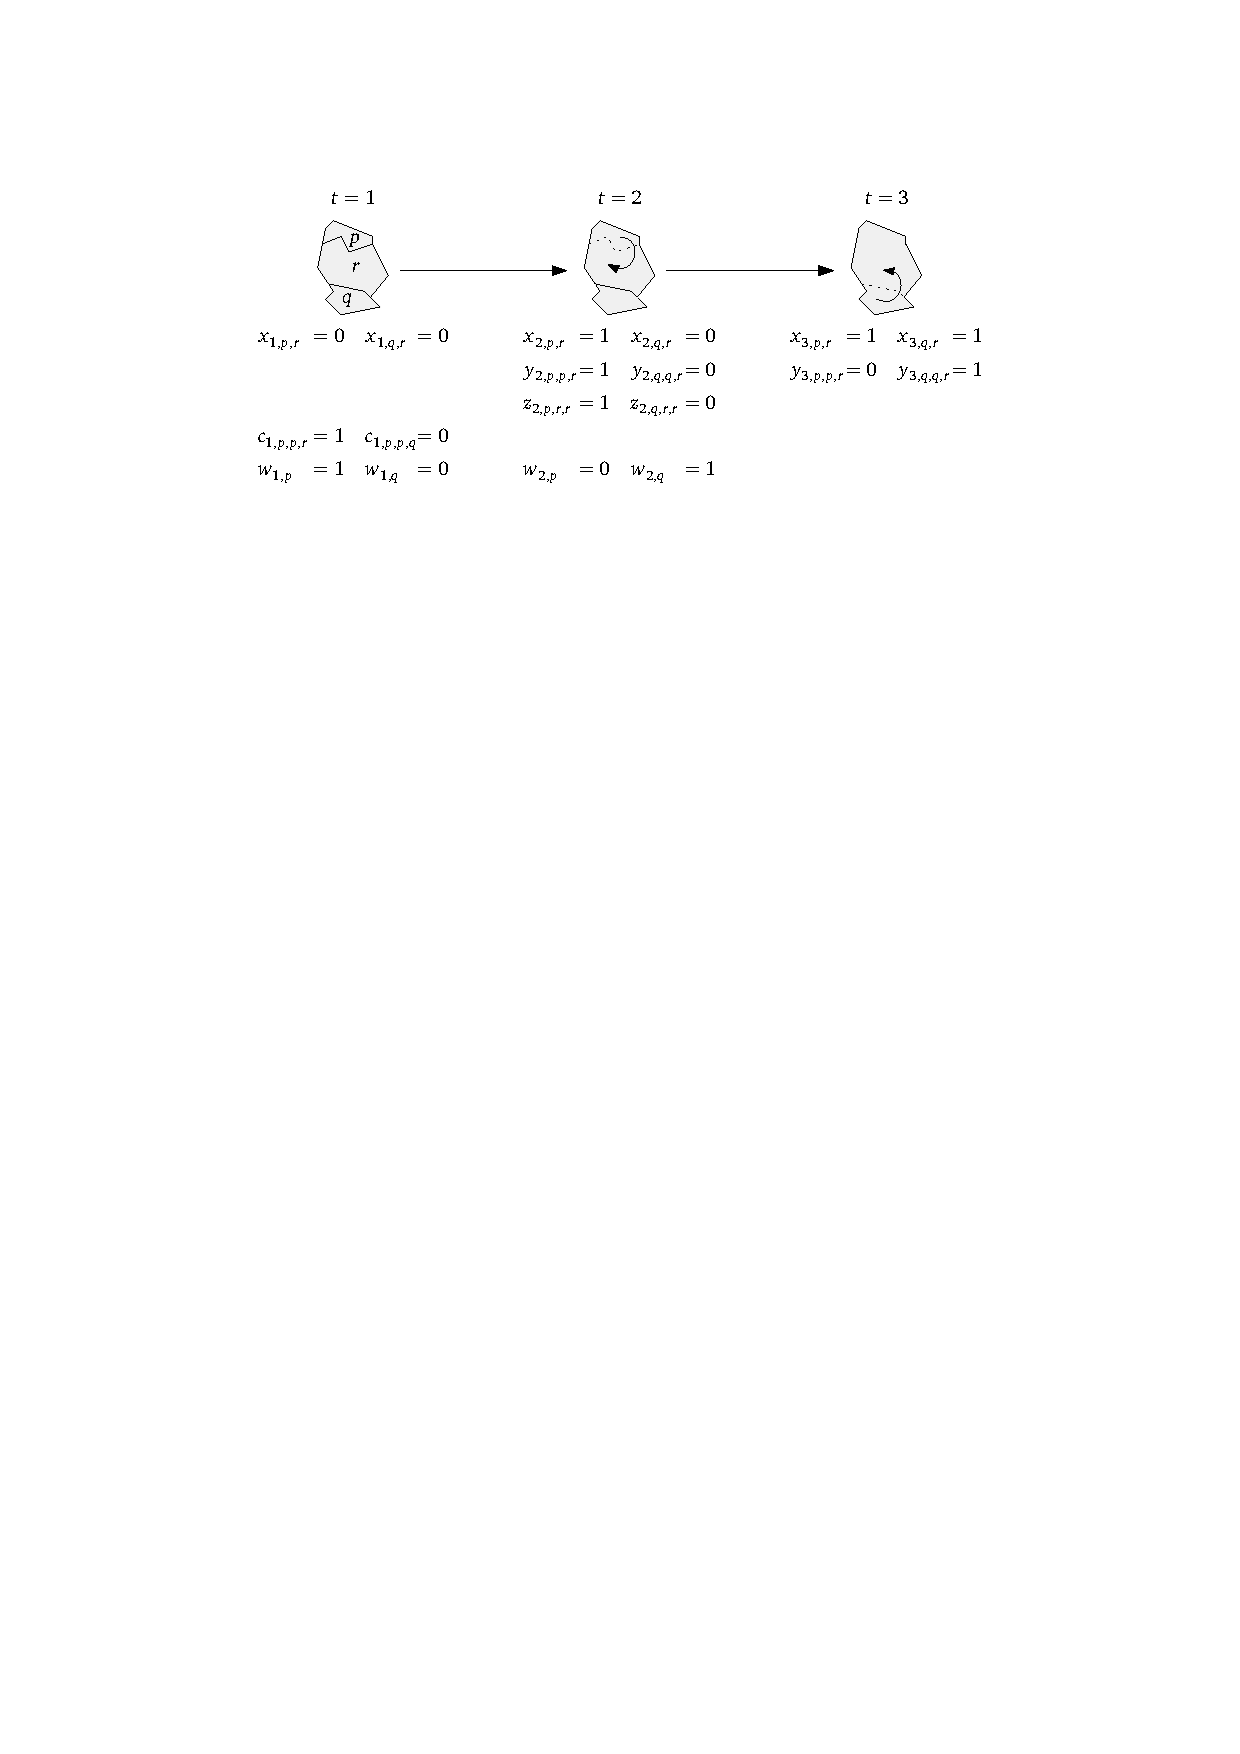
\includegraphics[page=1]{AreaAgg_ILP}
\caption{Some examples of the five sets of variables 
	for our ILP, $x$, $y$, $z$, $c$, and~$w$.
	The arrows with curly arms show the aggregation steps,
    and the dotted lines represent 
	the removed boundaries by the aggregation steps.
	There are some blank spaces in the rows of the variables
    because there is no corresponding variable at the specific times.
}
\label{fig:AreaAgg_Variables}
\end{figure*}
We introduce the variable 
\begin{flalign*}
&\eqquadVariable
\embrd[V]{x_{t,p,r}} \in
\embld[U]{\{0,1\}} \qquad 
\forall t\in T, \forall p,r \in P&
\end{flalign*}
with the intended meaning~$x_{t,p,r}=1$ if and only if 
polygon $p$ is assigned to polygon $r$ at time $t$
(see \fig\ref{fig:AreaAgg_Variables} for some examples). 
If a polygon is a center at time~$t$, 
then the polygon must be assigned to itself, 
that is, $x_{t,r,r}=1$.


We use the second set of variables in order to compute the
cost of type change. We introduce
\begin{flalign*}
&\eqquadVariable
\embrd[V]{y_{t,p,o,r}} \in
\embld[U]{\{0,1\}} \qquad 
\forall t\in T\setminus \{1\}, \forall p,o,r \in P&
\end{flalign*}
with the intended meaning~$y_{t,p,o,r}=1$ if and only if 
polygon~$p$ is assigned to center~$o$ at time~$t-1$ 
and assigned to center~$r$ at time~$t$ 
(see \fig\ref{fig:AreaAgg_Variables}).
Specifically, case~$y_{t,p,o,o}=1$ means that
polygon~$p$ is assigned to the same center 
at times~$t-1$ and~$t$.

We need a third set of variables 
for computing the cost of length.
We introduce
\begin{flalign*}
&\eqquadVariable
\embrd[V]{z_{t,p,q,r}} \in
\embld[U]{\{0,1\}} \qquad 
\forall t\in T\setminus \{1,n\}, \forall p,q,r \in P&
\end{flalign*}
with the intended meaning~$z_{t,p,q,r}=1$ 
if and only if polygons~$p$ and~$q$ 
are both assigned to center~$r$ at time~$t$
($p$ and $q$ are in the same patch).
In this case, their common boundary should be removed
(see \fig\ref{fig:AreaAgg_Variables}).
When variable~$z_{t,p,q,r}=1$ and~$p=q$,
we define the length of their common boundary to be~$0$ 
because we shall not remove any.
Note that time $t\in T\setminus \{1,n\}$.
We do not need~$z_{t,p,q,r}$ for time~$t=1$ 
because there are no two polygons in the same patch.
Namely, it always holds~$z_{1,p,q,r}=0$, 
which does not help in our ILP.
We do not need~$z_{t,p,q,r}$ for time~$t=n$
because all the polygons will be in the same patch.
In this case, \eq$z_{n,p,q,r}=1$ always holds,
which does not help in our ILP, either.

We use a fourth set of variables
to guarantee contiguity of each patch. 
In other words, we aggregate two patches 
only when they are neighbors (adjacent).
We introduce
\begin{flalign*}
&\eqquadVariable
\embrd[V]{c_{t,p,o,r}} \in
\embld[U]{\{0,1\}} \qquad 
\forall t\in T\setminus \{n-1,n\}, 
\forall p,o,r \in P \text{~with}~o\ne r,&
\end{flalign*}
with the intended meaning~$c_{t,p,o,r}=1$ 
if and only if, at time~$t$,
polygon~$p$ is assigned to center~$o$, 
and~$p$ has a neighbor assigned to center~$r$
(see \figs\ref{fig:AreaAgg_Variables}
and~\ref{fig:AreaAgg_Variables_Neighbor} for examples).
We do not need variable~$c_{t,p,o,r}$ for time~$t=n-1$ 
because there are only two patches left, 
and they must be neighbors.

Our last set of variables is needed to 
enforce that
every aggregation step involves a smallest patch. 
We define
\begin{flalign*}
&\eqquadVariable
\embrd[V]{w_{t,o}} \in
\embld[U]{\{0,1\}} \qquad 
\forall t\in T\setminus\{n\}, \forall o \in P&
\end{flalign*}
with $w_{t,o}=1$ meaning if and only if, at time~$t$, 
patch~$o$ is the smallest patch that is involved 
in the aggregation step from time~$t$ to time~$t-1$
(see for example \fig\ref{fig:AreaAgg_Variables}).

In total, the number of variables
in our ILP formulation is~$O(n^4)$.

\begin{figure}[tb]
\centering
\includegraphics[page=2]{AreaAgg_ILP}
\caption{There are two patches, 
	which respectively use polygons~$o$ and~$r$ 
	as their centers.
	Polygons in the same patch 
	are separated by dotted lines.
	Polygon~$p$, in patch~$o$, 
	has two neighbors assigned to center~$r$,
	i.e., polygons~$q_1$ and~$q_2$.
	In this case, patches~$o$ and~$r$ are neighbors 
	and can be aggregated.
}
\label{fig:AreaAgg_Variables_Neighbor}
\end{figure} 


\subsection{Objective}
\label{sub:AreaAgg_objective}

We want to minimize a weighted sum of the two costs, 
the cost of type change and the cost of length
(analogous to \eq\ref{eq:g_2}).
That is, our objective is to
\begin{equation}
\label{eq:ilpcost}
\mathrm{minimize} \quad 
(1-\lambda)F_\mathrm{type} +\lambda F_\mathrm{lgth},
\nonumber
\end{equation}
where~$\lambda$, as in \eq\ref{eq:g_2}, 
is a parameter 
to assign importances 
of~$F_\mathrm{type}$ and~$F_\mathrm{lgth}$.
According to the cost introduced in
\sect\ref{sec:AreaAgg_f_type},
we compute the total cost of type change by
\begin{flalign*}
%\label{eq:F_type}
&\eqquadCost
\embrd[V]{F_\mathrm{type}} =
\sum_{t=2}^{n} \sum_{p\in P} \sum_{o\in P} \sum_{r\in P}
\left(\frac{a_p}{A_R} \cdot
\frac{d_\mathrm{type}\left(T(o),T(r)\right)}{d_\mathrm{type\_max}}\cdot 
y_{t,p,o,r}\right), & 
\end{flalign*}
where, similar to \eq\ref{eq:f_type}, 
$a_p$ is the area of polygon~$p$,
$A_R$ is the area of the region, 
and~$T(o)$ and~$T(r)$ are 
the types of centers (polygons)~$o$ and~$r$.


We also wish to minimize the overall interior lengths 
of all the intermediate subdivisions.
As discussed in \sect\ref{sec:AreaAgg_costlength},
we use the length of the interior boundaries 
as an alternative to compactness.
Recall that~$B(\Pstart)$ is the set of interior boundaries 
at time~$t=1$ (see \sect\ref{sec:AreaAgg_costlength}).
We sum up the normalized lengths of 
the remaining interior boundaries 
of all the intermediate subdivisions by
\begin{flalign}
\label{eq:F_length_raw}
&\eqquadCost
\embrd[V]{F_\mathrm{lgth}} =
\frac{1}{n-2} \sum_{t=2}^{n-1} 
\frac{\sum_{b\in B (\Pstart)} |b| - 
	\frac{1}{2} \sum_{p \in P}\sum_{q \in P}\sum_{r \in P} 
	\left(|b_{pq}|\cdot z_{t,p,q,r}\right)} {D(t)}, &
\end{flalign}
where variable~$b_{pq}$ represents the common boundary 
between polygons~$p$ and~$q$. 
We define the length of the common boundary to be~$0$
(i.e., $|b_{pq}|=0$) if $p=q$ 
because there is no boundary to be removed in this case.
Function~$D(t)$, defined by \eq\ref{eq:AreaAgg_Norm}, 
is used to normalize the cost of length.
As in \eq\ref{eq:f_length}, 
we use denominator~$n-2$ to balance 
between the cost of type change and the cost of length.
Integrating \eq\ref{eq:AreaAgg_Norm} 
into \eq\ref{eq:F_length_raw}, we have
\begin{flalign*}
%\label{eq:F_length}
&\eqquadCost
\embrd[V]{F_\mathrm{lgth}} =
\frac{n-1}{n-2} \sum_{t=2}^{n-1}
\left(
\frac{1}{n-t} -
\frac{\sum_{p \in P}\sum_{q \in P}\sum_{r \in P} 
	\left(|b_{pq}|\cdot z_{t,p,q,r}\right)}
{2(n-t)\sum_{b\in B (\Pstart)} |b| }
\right). &
\end{flalign*}




\subsection{Constraints}
\label{sub:AreaAgg_Constraints}

In order to formulate our aggregation problem as an ILP, 
we restrict the variables introduced in 
\sect\ref{sub:AreaAgg_variables} 
by setting up constraints.
Recall that the intended meaning 
of~$x_{t,p,r}=1$ is if and only if 
polygon~$p$ is assigned to center~$r$ at time~$t$. 
To realize this functionality,
our first constraint is that 
polygon~$p$ is assigned to exactly one center at time~$t$. 
To this end, we require that
\begin{flalign}
\label{eq:CstrOneCenter}
&\eqquadConstraintsX
\embrd{\sum_{r\in P} x_{t,p,r}} =\embld{1} 
\inquad \forall t \in {T}, \forall p \in P. &
\end{flalign}


The next constraint is that polygon~$r$ is available to be 
assigned by other polygons only when~$r$ is a center.
In our case, if polygon~$r$ is a center, 
then it must be assigned to itself,
that is, $x_{t,r,r}=1$.
If~$r$ is not a center, we have variable~$x_{t,r,r}=0$.
In either case, we have
\begin{flalign}
\label{eq:CstrAssign}
&\eqquadConstraintsX
\embrd{x_{t,p,r}} \leq \embld{x_{t,r,r}}
\inquad \forall t \in {T}, \forall  p, r \in P. &
\end{flalign}


Aggregating a patch into another one results in 
the number of centers decreasing by~$1$.
We achieve that exactly one patch 
is aggregated into another by specifying the number of centers
for each point in time, that is,
\begin{flalign}
%\label{eq:CstrCountCenter}
&\eqquadConstraintsX
\embrd{\sum_{r\in P} x_{t,r,r}} =
\embld{n-t+1} \inquad
\forall t \in {T}, &
\end{flalign}
where polygon $r$ is a center at time~$t$ if and only if 
$x_{t,r,r}=1$.

When a patch is aggregated into another one,
the center of the former will not be used as a center anymore.
Hence, we have
\begin{flalign}
\label{eq:CstrNoReappear}
&\eqquadConstraintsX
\embrd{x_{t,r,r}} \le 
\embld{x_{t-1,r,r}} \inquad 
\forall t \in {T}\setminus \{1\},
\forall r \in P.&
\end{flalign}


On the start map, 
there are some polygons with the goal type,~$T_\mathrm{goal}$
(see definition in \sect\ref{sec:AreaAgg_h_type}).
At time~$t=n$, all polygons are aggregated into one patch.
This patch must have type~$T_\mathrm{goal}$.
In other words, the center of this patch must be one of the 
polygons with type~$T_\mathrm{goal}$ on the start map:
\begin{equation}
\label{eq:CstrType}
\sum_{r\in P\colon T(r)=T_\mathrm{goal}}
x_{n,r,r}=1,
\end{equation}
where $T(r)$ is the type of polygon $r$ at time $t=1$.

Next, we restrict binary variable~$y_{t,p,o,r}$,
introduced in \sect\ref{sub:AreaAgg_variables}.  
Recall that the intended meaning of~$y_{t,p,o,r}=1$ 
is if and only if 
polygon~$p$ is assigned to center~$o$ at time~$t-1$ 
and to center~$r$ at time~$t$.
To enforce this, we use two types of constraints.

First, if polygon~$p$ is assigned 
to center~$o$ at time~$t-1$ ($x_{t-1,p,o}=1$)
and assigned to center~$r$ at time $t$
($x_{t,p,r}=1$), we have variable~$y_{t,p,o,r}=1$. 
This requirement is expressed by
\begin{flalign}
\label{eq:CstrY1}
&\eqquadConstraintsYZ
\embrd{y_{t,p,o,r}} \geq 
\embld{x_{t-1,p,o}+x_{t,p,r}-1} \inquad
\forall t \in {T} \setminus \{1\}, 
\forall p, o, r \in P.&
\end{flalign}

Second, if~$p$ is not assigned to~$o$ at~$t-1$ ($x_{t-1,p,o}=0$)
and/or~$p$ is not assigned to~$r$ at time~$t$ ($x_{t,p,o}=0$),
we have variable~$y_{t,p,o,r}=0$.
This requirement is expressed by
\begin{flalign}
\label{eq:CstrY2}
&\eqquadConstraintsYZ
\begin{array}{@{}l}
\embrd{y_{t,p,o,r}} \le \\
\embrd{y_{t,p,o,r}} \le 
\end{array}
\embld{\embshift
	\begin{array}{@{}l}
	x_{t-1,p,o} \\
	x_{t,p,r}
	\end{array}
	\bigg\} 
}
\inquad \embshift
\forall t\in T\setminus \{1\}, 
\forall	p,o,r \in P.&	
\end{flalign}



%Third, if centers $o$ and $r$ are identical, 
%then the center of polygon $p$ is not changed.
%In this case, $y_{t,p,o,r}=0$, which is presented by
%\begin{equation}
%\label{eq:CstrY3}
%y_{t,p,o,r}=0 \qquad
%\forall t \in {T} / \{n\}, 
%\forall p, o, r \in P.
%\end{equation}

In \sect\ref{sub:AreaAgg_variables},
we introduced binary variable~$z_{t,p,q,r}$.
Recall that the intended meaning of~$z_{t,p,q,r}=1$ 
is if and only if
polygons~$p$ and~$q$ are both in patch~$r$ at time~$t$.
To enforce this, we need three types of constraints.

First, if two polygons~$p$ and~$q$ are assigned 
to center~$r$ at time~$t$ ($x_{t,p,r}=1$ and~$x_{t,q,r}=1$),
we have variable~$z_{t,p,q,r}=1$. 
This requirement is expressed by
\begin{flalign}
\label{eq:CstrZ1}
&\eqquadConstraintsYZ
\embrd{z_{t,p,q,r}} \geq 
\embld{x_{t,p,r}+x_{t,q,r}-1} \inquad
\forall t \in T \setminus \{1,n\}, 
\forall p, q, r \in P.&
\end{flalign}

Second, at time~$t$, if~$p$ is not assigned to~$r$ ($x_{t,p,r}=0$)
and/or~$q$ is not assigned to~$r$ ($x_{t,q,r}=0$), 
we have variable~$z_{t,p,q,r}=0$. 
This requirement is expressed by
\begin{flalign}
\label{eq:CstrZ2}
&\eqquadConstraintsYZ
\begin{array}{@{}l}
\embrd{z_{t,p,q,r}} \le  \\
\embrd{z_{t,p,q,r}} \le 
\end{array} 
\embld{\embshift
	\begin{array}{@{}l}
	x_{t,p,r} \\
	x_{t,q,r}
	\end{array}
	\bigg\} 
}
\inquad \embshift
\forall t \in T \setminus \{1,n\}, 
\forall p, q, r \in P.&	
\end{flalign}

Third, we introduce an abbreviation that will be helpful to 
express
the last type of constraint involving variable~$z_{t,p,q,r}$:
\begin{flalign}
\label{eq:CstrZabbrv}
&\eqquadConstraintsYZ
\embrd{z_{t,p,q}} = 
\embld{\sum_{r \in P}z_{t,p,q,r}}
\inquad 
\forall t\in T \setminus \{1,n\}, 
\forall	p,q \in P,&
\end{flalign}
where the reason we do not need~$z_{t,p,q}$ for~$t=1$ or~$t=n$
is the same as for $z_{t,p,q,r}$
(see \sect\ref{sub:AreaAgg_variables}).
Variable~$z_{t,p,q}$ expresses whether, at time~$t$, 
polygons~$p$ and~$q$ are 
in the same patch ($z_{t,p,q}=1$) or not ($z_{t,p,q}=0$).
%
Note that 
constraints~(\ref{eq:CstrOneCenter}) and~(\ref{eq:CstrZ2}) 
ensure that polygons~$p$ and~$q$ can be assigned 
to one common center at most; therefore, we have~$z_{t,p,q} \le 1$.
We use our new variable~$z_{t,p,q}$
to express the following requirement: 
If two polygons have been aggregated into one patch, 
they will always be in the same patch 
at later times---although 
the center of their common patch may change. 
In other words,  
variable~$z_{t,p,q}$ is monotonically increasing
as a function of time~$t$:
\begin{flalign}
\label{eq:CstrTogether}
&\eqquadConstraintsYZ
\embrd{z_{t,p,q}} \ge 
\embld{z_{t-1,p,q}} \inquad
\forall t \in \{3,4,\ldots,n-1\},  
\forall p, q \in P.&
\end{flalign}

Now we present our constraints of 
ensuring contiguity inside a patch.
This problem has received considerable attention 
in integer linear programming.
Usually, a subdivision is represented by a graph
(see \fig\ref{fig:AreaAgg_Variables_Graph}).
%
\textcite{Zoltners1983Territory} regarded each node as a center.
For each center, they found a shortest path 
to each of the other nodes.
Then, they required that a center can be assigned 
by a node only if 
at least one immediate predecessor of the node 
in the shortest path had been assigned to the center.
Although this requirement makes 
their problem easier to be solved,
it excludes many feasible patches.
%
\textcite{Williams2002Contiguous} 
built an optimal spanning tree for the nodes.
In order to ensure contiguity, 
the method picks a user-specified number of nodes that constitute 
an optimal subtree of the previously built spanning tree.
%
For a given center, \textcite{Cova2000_Contiguity} 
were able to find all the contiguous patches.
In their method, when a node is to be assigned to a center, 
a path from the node to the center was demanded 
that each node of the path is assigned to the center.
%
Similarly, \textcite{Shirabe2005Contiguity} modeled 
the contiguity problem as a network flow.
He required that there must be a path so that 
some fluid can flow from a node to a sink (center).
%
\textcite{Oehrlein2017Aggregation} utilized a method based 
on \emph{vertex separators}.	
Given center~$r$ and node~$p$, 
a separator is a set of nodes
such that any path from~$r$ to~$p$ 
will contain at least one node of the set.
The contiguity between center~$r$ and node~$p$ is ensured 
if each of the separators contains 
at least one node assigned to the center.
%
The last four ideas can be adapted into our method
as we do not wish to exclude any possible solutions.
However, we use an idea
that is more intuitive for our problem
since we aggregate step by step.


We aggregate two patches only if they are neighbors.
To ensure this, we need binary variable~$c_{t,p,o,r}$
introduced in \sect\ref{sub:AreaAgg_variables}.
Recall that the intended meaning of~$c_{t,p,o,r}=1$ 
is if and only if, at time~$t$, 
polygon~$p$ of patch~$o$ has 
at least one neighboring polygon in patch~$r$.
To enforce this behavior of~$c_{t,p,o,r}$, 
we need four types of constraints.

First, polygon~$p$ must actually be assigned 
to center~$o$ at time~$t$ ($x_{t,p,o}=1$).
In contrast, if~$p$ is not assigned to~$o$ ($x_{t,p,o}=0$),
then variable~$c_{t,p,o,r}$ is impossible to tell
if patch~$o$ and patch~$r$ are neighbors.
In this case, we must not aggregate the two patches ($c_{t,p,o,r}=0$);
otherwise, we may end up having noncontiguous patches.
As a result,
\begin{flalign}
\label{eq:CstrC_Part}
&\eqquadConstraintsC
\begin{array}{@{}l}
\embrd[C]{c_{t,p,o,r}} \le  \\
\embrd[C]{} %an empty place
\end{array} 
\embld[D]{\embshift
	\begin{array}{@{}l}
	x_{t,p,o} \\
	~ %an empty place
	\end{array}
}
\inquadC \embshift
\begin{array}{@{}l}
\forall t 	 \in T\setminus \{n-1,n\},\\
\forall p, o, r \in P \text{~with}~o\ne r.
\end{array} &	
\end{flalign}

Second, at time~$t$, at least one of polygon~$p$'s neighbor(s),
say, polygon~$q$ has to be assigned to center~$r$ ($x_{t,q,r}=1$).
If not, then variable~$c_{t,p,o,r}$ is impossible to tell
if patches~$o$ and $r$ are neighbors.
Analogous to the condition of constraint~(\ref{eq:CstrC_Part}),
we have
\begin{flalign}
\label{eq:CstrC_Neighbor}
&\eqquadConstraintsC
\begin{array}{@{}l}
\embrd[C]{c_{t,p,o,r}} \le  \\
\embrd[C]{} %an empty place
\end{array} 
\embld[D]{\embshift
	\begin{array}{@{}l}\displaystyle
	\sum_{q\in N_\mathrm{nbr}(p)} x_{t,q,r} \\
	~ %an empty place
	\end{array}
}
\inquadC \embshift
\begin{array}{@{}l}
\forall t 	 \in T\setminus \{n-1,n\},\\
\forall p, o, r \in P \text{~with}~o\ne r,
\end{array} &	
\end{flalign}
where~$N_\mathrm{nbr}(p)$ represents 
the set of polygons adjacent to~$p$.


Third, if polygon~$p$ is in patch~$o$ ($x_{t,p,o}=1$)
and~$p$ has at least one neighbor, say, 
polygon~$q$ in patch~$r$ ($x_{t,q,r}=1$),
then we must enforce variable~$c_{t,p,o,r}=1$
(according to the definition of this variable).
We have
\begin{flalign}
\label{eq:CstrC_Positive}
&\eqquadConstraintsC
\begin{array}{@{}l}
\embrd[C]{c_{t,p,o,r}} \ge  \\
\embrd[C]{} %an empty place
\end{array} 
\embld[D]{\embshift
	\begin{array}{@{}l}
	x_{t,p,o} + x_{t,q,r} -1 \\
	~ %an empty place
	\end{array}
}
\inquadC \embshift
\begin{array}{@{}l}
\forall t 	 \in T\setminus \{n-1,n\},\\
\forall p, o, r \in P \text{~with}~o\ne r,
\forall q \in N_\mathrm{nbr}(p).
\end{array} &	
\end{flalign}


Fourth, if we aggregate patch~$o$ into patch~$r$
from time~$t-1$ to time~$t$, 
we have variable~$y_{t,o,o,r}=1$
(see the definition of this variable 
in \sect\ref{sub:AreaAgg_variables}).
In this case, we must make sure that 
the two patches are actually neighbors at time~$t-1$.
That is to say, at least one of patch~$o$'s polygons 
has at least one neighbor in patch~$r$ at time~$t-1$.
If not, we have~$y_{t,o,o,r}=0$.
That is, it holds
\begin{flalign}
\label{eq:CstrC_Agg}
&\eqquadConstraintsC
\embrd[C]{y_{t,o,o,r}} \le 
\embld[D]{\sum_{p\in P} c_{t-1,p,o,r}} \inquadC
\forall t 	 \in T\setminus \{1,n\},  
\forall o, r \in P \text{~with}~o\ne r.&
\end{flalign}


If we do not require that 
each aggregation step must involve a smallest patch,
then we only need constraints
(\ref{eq:CstrOneCenter})--(\ref{eq:CstrC_Agg})
and variables~$x_{t,p,r}$, $y_{t,p,o,r}$, $z_{t,p,q,r}$,
and~$c_{t,p,o,r}$.
If we insist on involving a smallest patch at each step,
then we need more variables and more constraints.

\subsubsection{Aggregation involving a smallest patch}
In order to make sure that 
each of our aggregation steps involves a smallest patch,
we need another type of variable,~$w_{t,o}$.
Recall that the intended meaning of~$w_{t,o}=1$ is 
if and only if 
polygon~$o$ is the center of 
a smallest patch at time~$t$.
We will use this to enforce that
this patch is involved in the aggregation step 
from time~$t$ to~$t+1$.
At any time~$t$, 
we pick exactly one smallest patch (there can be many) 
and aggregate it with one of its neighbors;
we do not care whether or not the neighbor is a smallest one.
Therefore, we have
\begin{flalign}
\label{eq:CstrSOneSmallest}
&\eqquadConstraintW
\embrd[S]{\sum_{o\in P}w_{t,o}} =
\embld[T]{1} \inquad 
\forall t \in {T}\setminus \{n\}.&
\end{flalign}

Assume that patch~$o$ is the smallest patch
involved in the aggregation step from~$t$ to~$t+1$
and that we are aggregating patch~$o$ and another patch, say,~$r$.
There can be two cases.
We aggregate~$o$ into~$r$ 
or aggregate~$r$ into~$o$.
In the first case, we have variable~$y_{t+1,o,o,r}=1$,
and, in the second case, we have~$y_{t+1,r,r,o}=1$.
Either of the two cases implies 
that polygon~$o$ is indeed a center at time~$t$, 
that is,~$x_{t,o,o} =1$.
In order to enforce that
the aggregation step involves patch~$o$ and another patch,
we must make sure~$y_{t+1,o,o,r}=1$ or~$y_{t+1,r,r,o}=1$
when~$w_{t,o}=1$.
Consequently, we use the constraint
\begin{flalign}
\label{eq:CstrSInvolveSmallest}
%\displaystyle doesn't work for \setminus
%if we do \embld{\sum_{r\in P \setminus \{o\}}
&\eqquadConstraintW
\embrd[S]{w_{t,o}} \le 
\embld[T]{\displaystyle\sum_{r\in P \setminus \{o\}} 
\left(y_{t+1,o,o,r} +y_{t+1,r,r,o}\right)} \inquad
\forall t \in {T}\setminus \{n\}, 
\forall o \in P. &
\end{flalign}

Now we need to make sure that
patch~$o$ with $w_{t,o}=1$ is indeed 
a smallest patch at time~$t$.
We define variable~$A_{t,r}$ as the area of 
patch~$r$ at time~$t$. 
That is, we have
\begin{flalign*}
&\eqquadConstraintW
\embrd[S]{A_{t,r}} = 
\embld[T]{\sum_{p\in P} a_p \cdot x_{t,p,r},} &
\end{flalign*}
where~$a_p$ is the area of polygon~$p$ 
and, as viewed by the ILP, is a constant.
Area~$A_{t,r}$ is positive 
if and only if polygon~$r$ is a center at time~$t$ ($x_{t,r,r}=1$).
We define constant~$M$ as a very large number
to help us construct the corresponding constraints.
It suffices to set~$M$ to 
the area of the whole region, 
i.e., $M=A_R$ (see \eq\ref{eq:f_type}). 
We require
%\begin{flalign}
%\label{eq:CstrSIndeedSmallest}
%&\eqquadConstraints
%\embrd[S]{A_{t,o} - M(1-w_{t,o})} \le
%\embld[T]{A_{t,r}+M(1-x_{t,r,r})} \inquad
%\forall t 	 \in {T}\setminus \{n\}, 
%\forall o, r \in P \text{~with}~o\ne r. &
%\end{flalign}
%\begin{flalign}
%\label{eq:CstrSIndeedSmallest_Remove}
%&\eqquadConstraintW
%\embrd[S]{A_{t,o}} -
%\embld[T]{M(1-w_{t,o}) \le A_{t,r}+M(1-x_{t,r,r})} \inquad
%\forall t 	 \in {T}\setminus \{n\}, 
%\forall o, r \in P \text{~with}~o\ne r. &
%\end{flalign}
%\begin{equation}
%A_{t,o} - M(1-w_{t,o}) \le A_{t,r}+M(1-x_{t,r,r}) \inquad
%\forall t 	 \in {T}\setminus \{n\}, 
%\forall o, r \in P \text{~with}~o\ne r.
%\end{equation}
\begin{flalign}
\label{eq:CstrSIndeedSmallest}
&\eqquadConstraintW
\begin{array}{@{}l}
\embrd[S]{A_{t,o}- M(1} -\\
\embrd[S]{} %an empty place
\end{array} 
\embld[T]{\embshift
	\begin{array}{@{}l}
	w_{t,o}) \le A_{t,r}+M(1-x_{t,r,r}) \\
	~ %an empty place
	\end{array}
}
\inquad \embshift
\begin{array}{@{}l}
\forall t 	 \in T\setminus \{n\},\\
\forall o, r \in P \text{~with}~o\ne r.
\end{array} &	
\end{flalign}
This constraint takes effect only when~$w_{t,o}=1$ 
and~$x_{t,r,r}=1$, which indicates that 
patch~$o$ is smaller than or equal to 
all the other existing patches at time~$t$.

In order to compute an aggregation sequence 
involving a smallest patch at each step, 
we need all the five types of variables and all the
constraints~(\ref{eq:CstrOneCenter})--(\ref{eq:CstrSIndeedSmallest}).
In total, the number of constraints is~$O(n^4)$.

\section{Case Study}
\label{sec:AreaAgg_CaseStudy}
We have implemented our methods 
based on C\# (Microsoft Visual Studio~2017) 
and ArcObjects SDK~10.6.0.
We used the IBM ILOG
CPLEX Optimization Studio~12.6.3.0 to solve our ILP.
Our prototype is open access on GitHub\footnote{%
\url{https://github.com/IGNF/ContinuousGeneralisation},
Accessed: Jun 18, 2018.}.
We ran our case study
under 64-bit Windows~10 
on Intel(R) Core(TM) i7-6700 CPU @~$3.40\,$GHz with~$4$ cores;
the computer has $16\,$GB RAM.
We measured processing time 
by the built-in C\# class \emph{Stopwatch}.
As required by ArcObjects SDK~10.6.0,
we specified our program to run on the~$32$-bit platform. 
We added a post-build task about ``largeaddressaware''
in Microsoft Visual Studio so that 
we were able to use up to~$3\,$GB of the 
main memory\footnote{The details of the setting can be found at \url
{http://stackoverflow.com/questions/2597790/can-i-set-largeaddressaware-from-within-visual-studio},
Accessed: Nov 1, 2017.}.
Our CPLEX version may declare an optimal solution
while it is not really optimal.
To fix this problem, we had to disable 
both primal and dual presolve 
reductions\footnote{For more details about the problem, see
\url{http://www-01.ibm.com/support/docview.wss?uid=swg1RS02094},
Accessed: Nov 12, 2017.}.

We tested our method on a dataset 
from the German topographic database ATKIS DLM~50. 
The dataset represents the place 
``Buchholz in der Nordheide'' at scale~$1:50{,}000$. 
Our start map is the result of collapsing areas 
by \citet[\chap6]{haunert2008f}.
The start map has~$5{,}537$ polygons. 
Our goal map was generalized from the start map 
by~\citet{HaunertWolff2010AreaAgg}, setting the scale 
to~$1:250{,}000$ (see \fig\ref{fig:AreaAgg_Data}). 
The goal map has~$734$ polygons, 
which means that there are~$N=734$ regions.
The distribution of region sizes is shown in 
\fig\ref{fig:AreaAgg_NumRegion}.
%
We used a tree-based method introduced by 
\citet{Rada1989SemanticMetric} 
to define the distances of the types;
the distance is the ``number of edges'' that
we need to travel from one node to another node in the tree of 
type hierarchy\footnote{More information 
    about land-cover types can be found at 
	\url{http://www.atkis.de/dstinfo/dstinfo2.dst_gliederung},
	Accessed: Nov 1, 2017.}
(see \fig\ref{fig:AreaAgg_TypeDistances}). 
For example, the distance from type \emph{village}
to type \emph{fence} is~$2$, 
to type \emph{street} is~$4$, and
to type \emph{farm land} is~$6$.
In this tree, the maximum distance is~$6$, 
which means~$d_\mathrm{type\_max}=6$ for \eq\ref{eq:f_type}.
According to \citet{Rada1989SemanticMetric}, 
the resulting cost function for type change is a metric.


\begin{figure}[tb]
%\captionsetup[subfigure]{labelformat=empty}
\begin{subfigure}[b]{.49\textwidth}
\centering
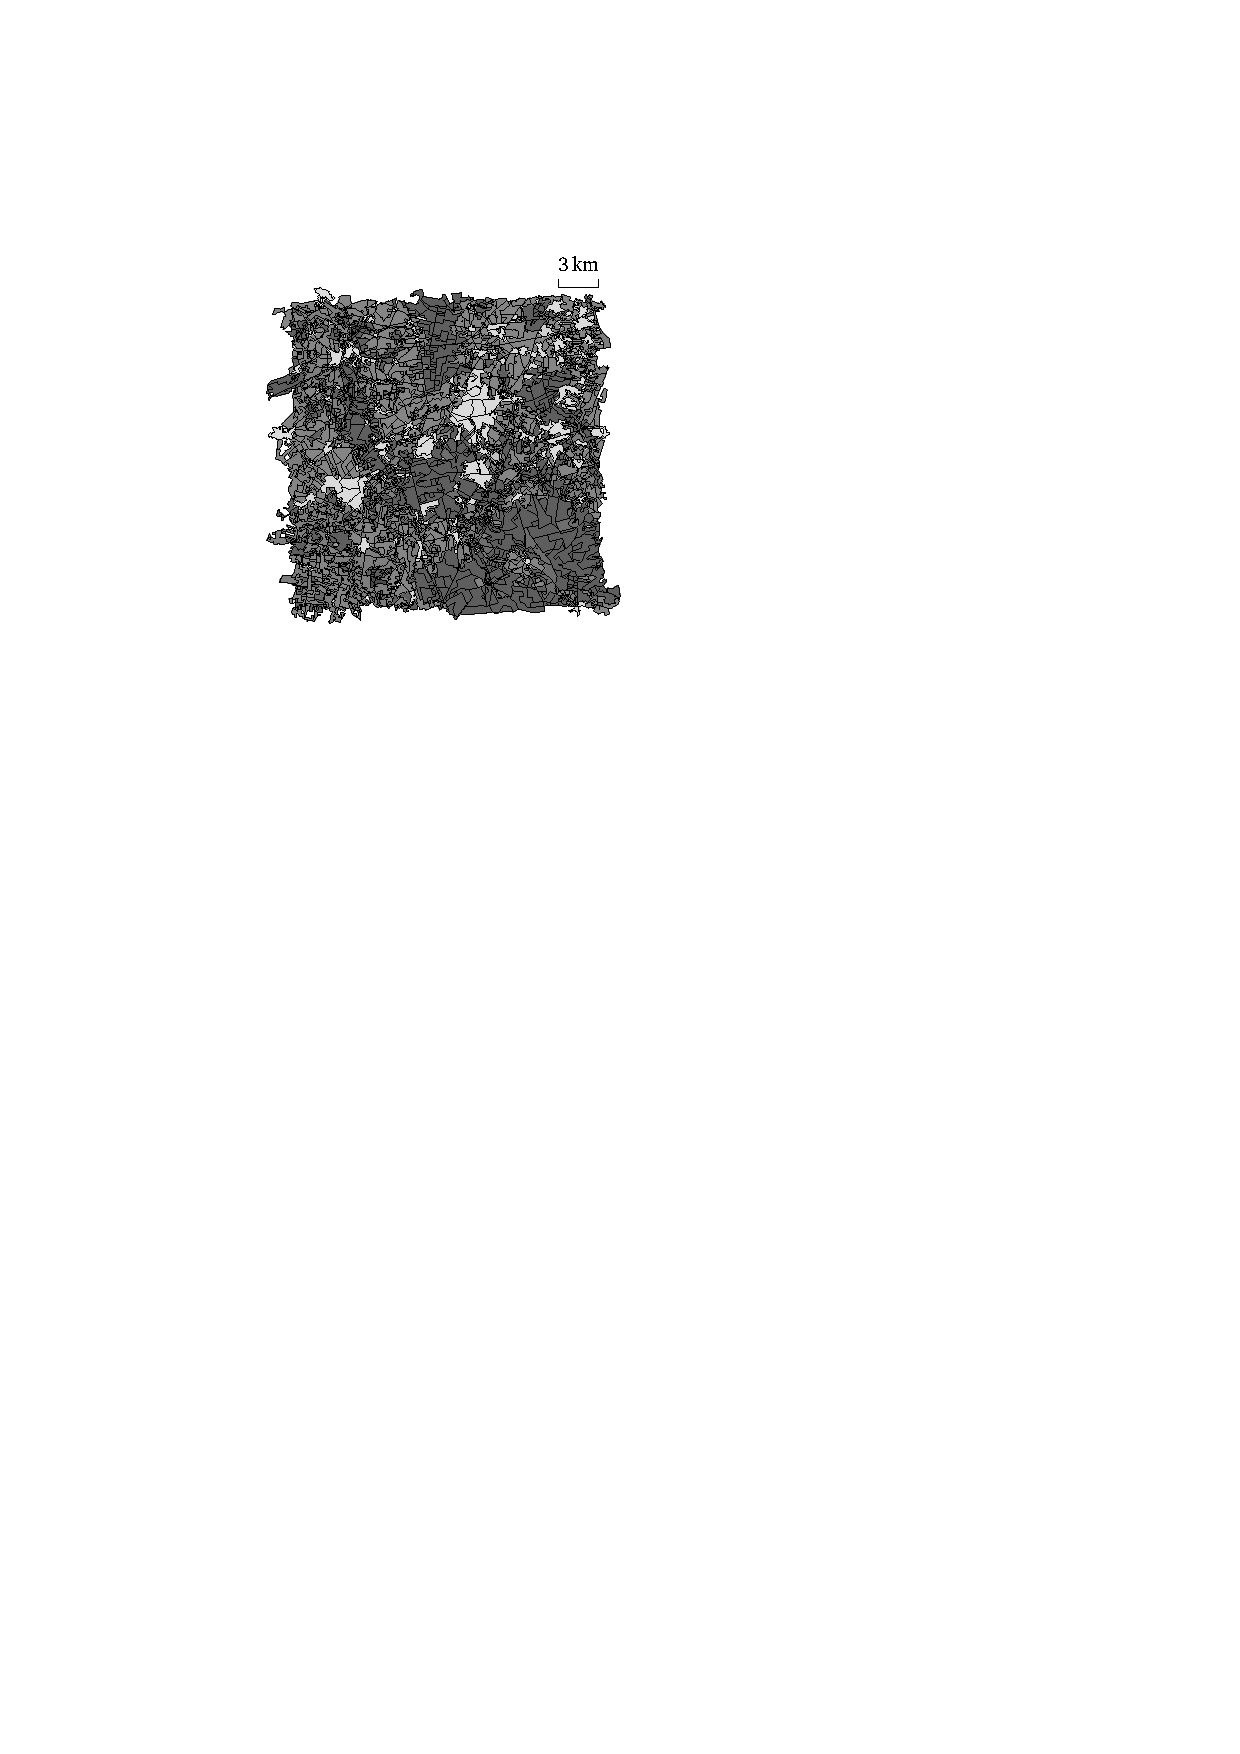
\includegraphics[page=1]{AreaAgg_Data}
\caption{Start map, $5{,}537$ polygons, \\
	at scale $1:50{,}000$}
\end{subfigure}
\hfill
\begin{subfigure}[b]{.49\textwidth}
\centering
\includegraphics[page=2]{AreaAgg_Data}
\caption{Goal map, $734$ polygons, \\
	at scale $1:250{,}000$}
\end{subfigure}
%
%It doesn't work to directly use 
%\vspace{\baselineskip} for subfigures.
\par\vspace{\baselineskip} %Leave a gap	figures
%
\begin{subfigure}{\textwidth}
\centering
\includegraphics[page=3]{AreaAgg_Data}
\caption{The 20 land-cover types appearing in our data}
\end{subfigure}
\caption{The data of our case study.}
\label{fig:AreaAgg_Data}
\end{figure}

\begin{figure}[tb]
\centering
\includegraphics[page=4]{AreaAgg_Data}
\caption{Distribution of the region sizes:
	the $y$-axis shows how many regions 
	of a given size range are contained in our dataset.}
\label{fig:AreaAgg_NumRegion}
\end{figure}

\begin{figure}[tb]
\centering
\includegraphics[page=5]{AreaAgg_Data}
\caption{The tree of type hierarchy used in our case study.
	For example, the distance between 
	types \emph{village} and \emph{farm land} is~$6$.}
\label{fig:AreaAgg_TypeDistances}
\end{figure}

\subsection{Using Costs of Type Change and Compactness}
\label{sec:AreaAgg_CaseStudy1}

As illustrated in \sect\ref{sec:AreaAgg_Combining},
we compare the \Astar algorithm and 
the greedy algorithm using $g_1(\Pnode)$,
which is a combination of the costs 
of type change and compactness (see \eq\ref{eq:g_1}).
For \Astar, we overestimated 
whenever we could not find a solution after 
having visited~$W$ nodes 
(see \sect\ref{sec:AreaAgg_AStar}).
We tried~$W=200{,}000$ and~$W=400{,}000$
(if we could use more main memory, 
then we could test by using some larger~$W$). 
The results are shown in 
Table~\ref{tab:AreaAgg_CaseStudy1_Statistics}.
%
Comparing to \Astar, 
the greedy algorithm visited 
fewer nodes and arcs in graph~$G_\mathrm{S}$ 
and used much less time.
However, \Astar managed to find solutions with 
lower total cost,~$117.3$ (or~$117.2$), 
which is~$2.8\%$ less than 
the total cost of the greedy algorithm,~$120.7$.
%
When~$W=200{,}000$, we are sure that 
we have found optimal solutions 
for~$702$ of the~$734$ regions ($95.6\%$),
while the greedy algorithm solved 
only~$408$ ($55.6\%$) to optimality;
see column \#OS in 
Table~\ref{tab:AreaAgg_CaseStudy1_Statistics}.
For the other~$32$ regions, 
both algorithms have found feasible solutions 
(see column \#FS in 
Table~\ref{tab:AreaAgg_CaseStudy1_Statistics}).
Although some of the feasible solutions may also be optimal,
we cannot verify that only from the cost values.


\begin{table*}[tb]
\caption{A comparison of the greedy algorithm and \Astar		
	when using cost function~$g_1$ (see \eq\ref{eq:g_1}).
	For \Astar, we used two settings, 
	i.e.,~$W=200{,}000$ and~$W=400{,}000$.
	%
	Column~\#OS shows the numbers of regions 
    that we obtained optimal solutions.   
	%
	Column~\#FS presents 
    the numbers and the percentages of regions (out of~$N=734$) 
    that we obtained feasible (non-optimal) solutions.
	%
	Variable~$k_\mathrm{sum}$ is 
	the total number of repetitions.
	%
	Columns~\#nodes and~\#arcs are the total 
	numbers of nodes and arcs that \Astar visited  
	(for instances where we needed overestimation, 
	only the final attempt was counted).
	%
	Columns~$\sum g_\mathrm{type}$, $\sum g_\mathrm{comp}$, 
	and~$\sum g_1$
	respectively denotes the sums of~$g_\mathrm{type}(\Pgoal)$,
	$g_\mathrm{comp}(\Pgoal)$, and~$g_1(\Pgoal)$ 
	over all the~$734$ instances 
	(see \eqs\ref{eq:g_type}, \ref{eq:g_comp}, 
	and~\ref{eq:g_1}).
	%
	The percentage in the \emph{Time}
	column is the fraction of the runtime 
    spent on solving the instances
	that we obtained feasible solutions.
    For \Astar, the time needed for overestimation
    is included.
}
\label{tab:AreaAgg_CaseStudy1_Statistics}
\centering
\fontsize{9}{11}\selectfont %for my thesis; should before \setlength{\tabcolsep}{0.7ex}
\setlength{\tabcolsep}{0.7ex}
\begin{tabular}{lRRRCCCCCd{3.7}}
\toprule
\multicolumn{1}{l}{Methods} &
\multicolumn{1}{c}{\#OS} &
\multicolumn{1}{c}{\#FS} &
\multicolumn{1}{r}{$k_\mathrm{sum}$} &  
\multicolumn{1}{c}{\#nodes} & 
\multicolumn{1}{c}{\#arcs} & 
\multicolumn{1}{c}{$\sum g_\mathrm{type}$} & 
\multicolumn{1}{c}{$\sum g_\mathrm{comp}$} & 
\multicolumn{1}{c}{$\sum g_1$} & 
\multicolumn{1}{c}{Time (min)} \\ 
\midrule
Greedy 	& 408 
&326~(44.4\%) 
&             &5.5\cdot 10^3   &4.8\cdot 10^3   
&53.2         &188.2           &120.7           &0'1~(74.6\%)\\
%
%
\AstarTwo	& 702 
&  32~(\parbox{\widthof{$4$}}{$\,$}$4.4\%$) 
& 102 &  3.6\cdot 10^6 &    5.7\cdot 10^6	
& 51.4 & 183.2 & 117.3 & 51'6~(93.2\%)\\
%
%
\AstarFour	& 704 
&  30~(\parbox{\widthof{$4$}}{$\,$}$4.1\%$)
&  89 &  6.5\cdot 10^6 &    9.8\cdot 10^6
& 51.4 & 183.1 & 117.2 & 93'1~(95.5\%)
\\ \bottomrule			
\end{tabular}
\end{table*}


In accordance with \sect\ref{sec:AreaAgg_AStar}, 
for region with ID~$i$ 
we define~$k_i$ as the least number of repetitions 
that we do to find a feasible solution. 
We define the total number of repetitions 
as~$k_\mathrm{sum}=\sum_{i=1}^N k_i$, 
where~$N=734$ is the number of the regions.
After increasing~$W$ to~$400{,}000$, 
\Astar found optimal aggregation sequences 
for only two more regions, 
but $k_\mathrm{sum}$ decreased quite a bit, 
from~$102$ to~$89$. 
The numbers of regions that needed certain
overestimation steps are shown in 
\fig\ref{fig:AreaAgg_OverStats}. 
Besides, \Astar visited more arcs and nodes, 
used more time, 
but got (slightly) less cost when increasing~$W$ to~$400{,}000$.
Although the number of regions 
that needed overestimation is relatively small, 
\Astar spent most of the running time 
on those few regions:~$4.4\%$ and~$4.1\%$ of the regions 
caused~$93.2\%$ and~$95.5\%$ of the total running time, 
respectively 
(see Table~\ref{tab:AreaAgg_CaseStudy1_Statistics}).

\begin{figure}[tb]
\centering
\includegraphics[page=2]{AreaAgg_CaseStudy1_Plot}
\caption{The numbers of regions where \Astar was 
	forced to use the given overestimation parameters
	in order to find a solution 
	without exploring more than 
	$W \in \{200{,}000;~400{,}000\}$ 
	nodes of the subdivision graph.}
\label{fig:AreaAgg_OverStats}
\end{figure}

The details of some regions are presented in 
Table~\ref{tab:CostsInDetail}.
According to the entries with overestimation factor $K_i=0$, 
we often have 
ratios~$R_\mathrm{type}=1$ and~$R_\mathrm{comp}>1$.
When factor~$K_i=0$, we did not overestimate for region~$i$.
The estimated cost must be smaller or equal to the exact cost,
which results in~$R_\mathrm{type}\ge 1$ 
and~$R_\mathrm{comp}\ge 1$.
Ratio~$R_\mathrm{type} = 1$ means that our estimation for the 
cost of type change is the best.
A larger~$R_\mathrm{comp}$ means 
a poorer estimation for the cost of shape.

\begin{table*}[tb]
\caption{The costs in detail of some regions, 
	where~$W=200{,}000$.  
	Parameters~$n$ and~$m$ are the numbers of patches and 
	adjacencies on the start map, respectively.
	Parameter $K$ is the overestimation factor, 
	defined in \sect\ref{sec:AreaAgg_Preliminaries}. 
	We evaluate the quality 
	of our estimations for type change and 
	compactness by listing the numbers~
	$R_\mathrm{type}=g_\mathrm{type}(\Pgoal)
	/h_\mathrm{type}(\Pstart)$ and~
	$R_\mathrm{comp}=g_\mathrm{comp}(\Pgoal)
	/h_\mathrm{comp}(\Pstart)$. 
	Note that if~$h_\mathrm{type}(\Pstart)=0$,
    then we have~$g_\mathrm{type}(\Pgoal)=0$; 
	in this case, we define~$R_\mathrm{type}=1$.
	The marked entries are discussed in the text.
}
\label{tab:CostsInDetail}
\centering
\includegraphics[page=3]{AreaAgg_CaseStudy1_Plot}
\end{table*}


According to columns~$n$ and~$K$ of \tab\ref{tab:CostsInDetail},
\AstarTwo managed to find optimal solutions 
for all the regions with fewer than~$15$ polygons,
and only found feasible solutions 
for any region with more than~$21$ polygons.
Among the~$702$ regions that 
\AstarTwo solved to optimality,
the greedy algorithm failed to 
find optimal solutions for~$294$ regions.
Solutions of the greedy algorithm cost
at most~$41.7\%$ more than 
solutions of \AstarTwo;
for region~$85$, the greedy algorithm yields 
a solution of cost~$0.777$, 
while the solution of \AstarTwo has cost~$0.548$
(see \fig\ref{fig:AreaAgg_CaseStudy1_Rg85}).
As the patches in the two sequences are the same,
the two results have the same cost of compactness.
The main difference is the choice of the first step, 
from~$8$ patches to~$7$.
When aggregating the smallest patch on the start map
with the surrounding patch,
our greedy algorithm chooses the type 
which is closer to the goal type.
In this case, the smallest patch has type~$5112$, and the 
surrounding one has~$2112$.
The type of the goal patch is~$4102$.
According to \fig\ref{fig:AreaAgg_TypeDistances},
type distances~$d_\mathrm{type}(5112,4102)=4$ and~$d_\mathrm{type}(2112,4102)=6$.
As a result, our greedy algorithm uses~$5112$ 
as the type for the new patch. 
This choice is a big mistake 
because the type of the largest patch on the start map
will have to be changed twice during the aggregation.
These changes cause a cost more than the sequence obtained by 
\AstarTwo, 
where the largest patch on the start map is changed to 
the target type directly.

Among the $32$~regions that 
\AstarTwo failed to solve optimally,
the greedy algorithm outperformed \AstarTwo 
for~$15$ regions ($46.9\%$).
%
Among these, solutions of the greedy algorithm 
cost at most~$15.9\%$ less than solutions of \AstarTwo;
for region~$543$, the greedy algorithm yields 
a solution of cost~$0.112$, 
while the solution of \AstarTwo costs~$0.134$. 
For this instance, 
\AstarTwo used overestimation parameter~$K=7$
(marked in \tab\ref{tab:CostsInDetail}).
\fig\ref{fig:AreaAgg_CaseStudy1_Rg543} shows 
some intermediate results obtained by
\AstarTwo and the greedy algorithm.
Interestingly, the two methods produced the same sequence until 
there were~$8$ patches left.
Then due to the overestimation, 
\AstarTwo did some bad moves
because the bad aggregation sequence still seemed better 
than other sequences.
In contrast, the greedy algorithm was looking for locally good 
aggregations.
%
Among the~$32$ regions that 
\AstarTwo failed to solve optimally,  
solutions of the greedy algorithm cost at most~$17.4\%$ 
more than solutions of \AstarTwo; 
for region~$155$, the greedy algorithm yields 
a solution of cost~$0.372$, while
the solution of \AstarTwo costs~$0.317$
(marked in \tab\ref{tab:CostsInDetail}).

Finally, an optimal aggregation sequence of region~$53$
(third-last row in \tab\ref{tab:CostsInDetail})
obtained by \AstarTwo
is shown in \fig\ref{fig:AreaAgg_CaseStudy1_Rg53}.

\begin{figure}[tb]
\centering
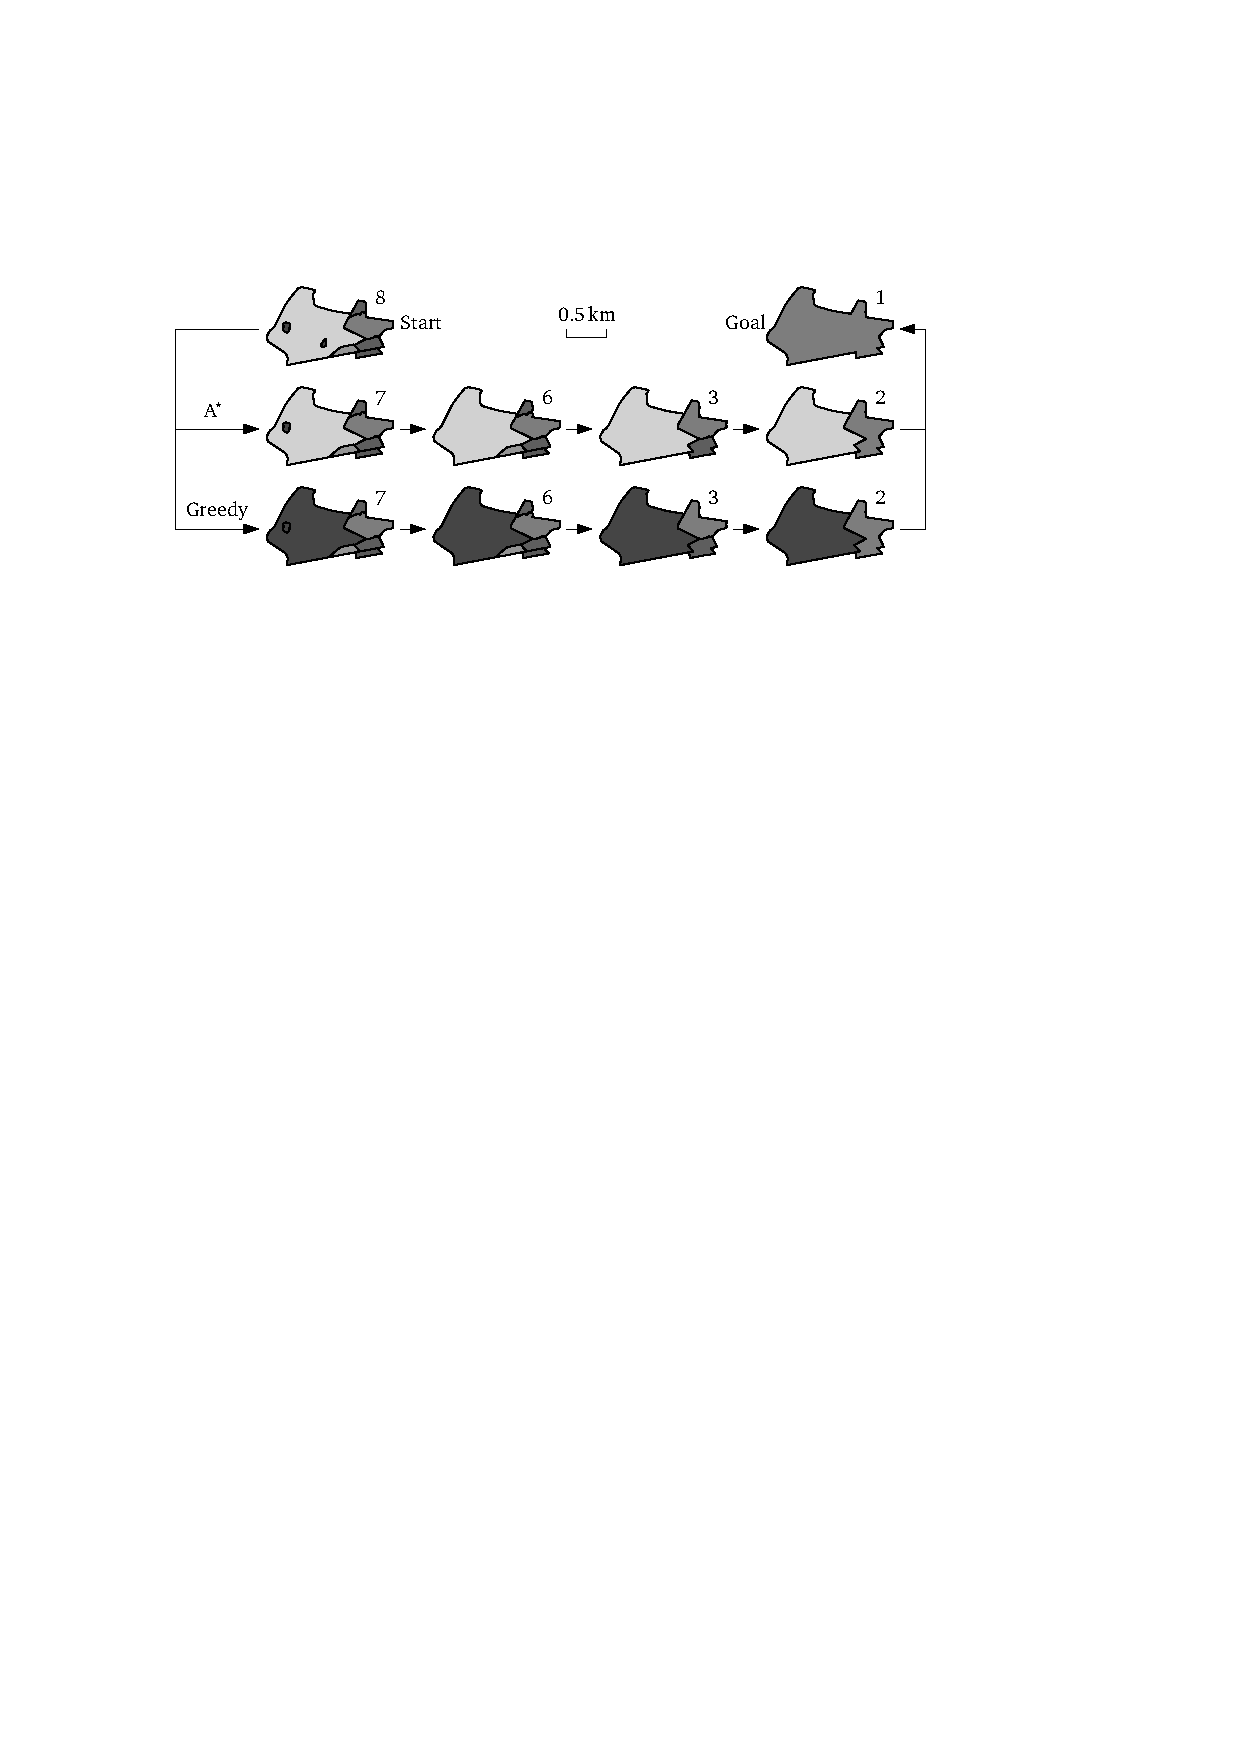
\includegraphics[page=1]{AreaAgg_CaseStudy1}
\caption{Aggregation sequences of region~$85$ 
	obtained by \Astar and the greedy algorithm.
	In order to save space, we did not show the results 
	when there are~$4$ or~$5$ patches, 
	which one can easily deduce.
	The numbers indicate the numbers of patches.
    %
    In the sequence obtained by \Astar, 
    the type of the largest polygon on the start map 
    changed only once, which is good; 
    while the type of the largest polygon changed twice 
    in the sequence obtained by the greedy algorithm.}
\label{fig:AreaAgg_CaseStudy1_Rg85}
\end{figure}

\begin{figure}[tb]
\centering
\includegraphics[page=2]{AreaAgg_CaseStudy1}
\caption{Some intermediate subdivisions of region~$543$ 
	obtained by \Astar and the greedy algorithm.
	In the sequence obtained by \Astar, 
	a pair of circles or a pair of squares indicates that
	the two parts are actually in the same patch.
	The numbers indicate the numbers of patches.
}
\label{fig:AreaAgg_CaseStudy1_Rg543}
\end{figure}


\begin{figure}[tb]
\centering
\includegraphics[page=3]{AreaAgg_CaseStudy1}
\caption{An optimal sequence of intermediate subdivisions 
	of region~$53$ obtained by \Astar 
	using the costs of type change and compactness.		 
	The numbers indicate the numbers of patches.		
}
\label{fig:AreaAgg_CaseStudy1_Rg53}
\end{figure}


%\todo[inline]{It turned out that the objective function $g$ 
%seems rather robust
%	against changes of~$\lambda$.  For region~77, we 
%	varied~$\lambda$ in
%	the range $\{0.1,0.5,0.9\}$, but the resulting aggregation 
%	sequences
%	stayed almost the same.  When we used even larger 
%	values 
%	for~$\lambda$ (e.g.,~$0.99$), the (good) influence of type 
%	change was mitigated 
%	and, as a
%	result, we needed to overestimate (with factor~$K=8$).}




\subsection{Using Costs of Type Change and Length}
\label{sec:AreaAgg_CaseStudy2}

We compare the greedy algorithm, \Astar, and ILP
using~$g_2(\Pnode)$,
a combination of the costs 
of type change and length (see \eq\ref{eq:g_2}).
For \Astar, we overestimated 
whenever we could not find a solution after 
having visited~$W=200{,}000$ nodes 
(see \sect\ref{sec:AreaAgg_AStar}).
The most time-consuming instance for \Astar was region~$94$,
for which \Astar took~$104.1\,$s (including repetitions)
to find a feasible solution 
with overestimation factor~$K=31$.
To avoid waiting too long,
we set the time limit to~$100\,$s 
for our ILP to run on one region.
Note that the time limit included
the time that our ILP used 
to set up the variables and constraints
(see \sects\ref{sub:AreaAgg_variables} 
and~\ref{sub:AreaAgg_Constraints}).
If no optimal solution was found in this time limit,
a feasible solution (if found) would be returned.
For some large instances, 
the ILP could not find any solution.

Using a similar format as in 
\tab\ref{tab:AreaAgg_CaseStudy1_Statistics},
we present the statistics in 
\tab\ref{tab:AreaAgg_CaseStudy2_Statistics}.
\Astar found optimal solutions 
for~$695$ of the~$734$ regions ($94.7\%$).
Again, it spent most of the running time 
on the few regions that needed 
overestimation:~$5.3\%$ of the regions 
caused~$92.3\%$ of the total running time.
The solutions by \Astar cost~$438.2$ in total, 
which is~$3.9\%$ less than~$455.8$, 
the total cost of the solutions by the greedy algorithm.

\begin{table*}[tb]
\caption{A comparison of the greedy algorithm, 
    the \Astar algorithm, and the ILP-based algorithm		
	when using cost function~$g_2$ (see \eq\ref{eq:g_2}).
	The notations are the same as in
	\tab\ref{tab:AreaAgg_CaseStudy1_Statistics}.
	%
	Columns~$\sum g_\mathrm{type}$, $\sum g_\mathrm{lgth}$, 
	and~$\sum g_2$
	respectively represent the sums of~$g_\mathrm{type}(\Pgoal)$,
	$g_\mathrm{lgth}(\Pgoal)$, and~$g_2(\Pgoal)$ 
	over all the~$734$ instances 
	(see \eqs\ref{eq:g_type}, \ref{eq:g_length}, 
	and~\ref{eq:g_2}).
}
\label{tab:AreaAgg_CaseStudy2_Statistics}
%	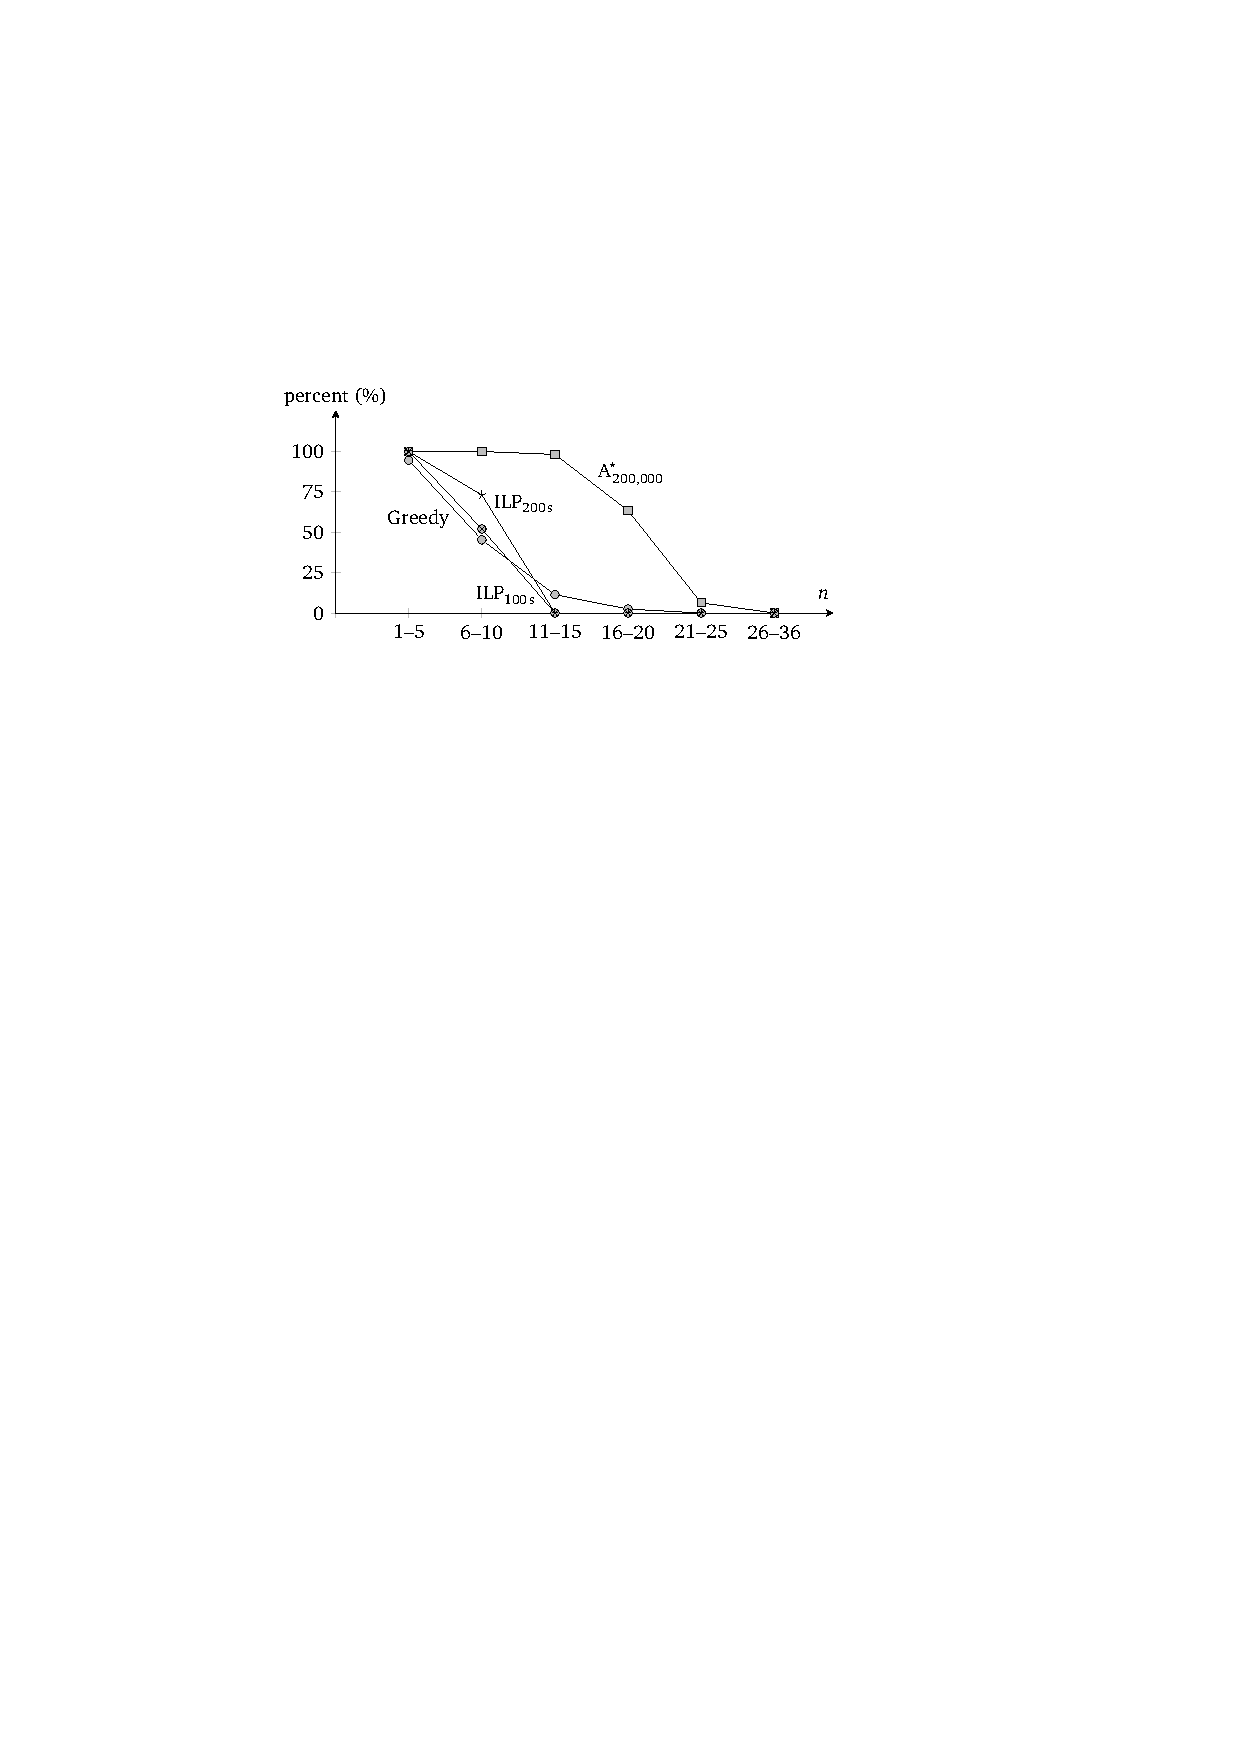
\includegraphics[page=1]{AreaAgg_CaseStudy2_Plot}
\centering
\fontsize{9}{11}\selectfont %for my thesis; should before \setlength{\tabcolsep}{0.7ex}
\setlength{\tabcolsep}{0.7ex}
\begin{tabular}{lRRRCCCCCd{3.7}}
\toprule
\multicolumn{1}{l}{Methods} &
\multicolumn{1}{c}{\#OS} &
\multicolumn{1}{c}{\#FS} &
\multicolumn{1}{r}{$k_\mathrm{sum}$} &  
\multicolumn{1}{c}{\#nodes} & 
\multicolumn{1}{c}{\#arcs} & 
\multicolumn{1}{c}{$\sum g_\mathrm{type}$} & 
\multicolumn{1}{c}{$\sum g_\mathrm{lgth}$} & 
\multicolumn{1}{c}{$\sum g_2$} & 
\multicolumn{1}{c}{Time (min)} \\ 
\midrule
Greedy 		 &430             
&304~(41.4\%)    
&            &5.5\cdot 10^3   &4.8\cdot 10^3   
&53.0        &858.5           &455.8           &0'1~(70.7\%)\\
%
%
\AstarTwo	& 695
& 39~(\parbox{\widthof{$4$}}{$\,$}$5.3\%$)	
& 150 	& 3.7\cdot 10^6 & 7.3\cdot 10^6 
& 52.0 	& 824.5 & 438.2 &44'8~(92.3\%)	\\
%
%
\ILPOne		& 449
& 69~(\parbox{\widthof{$4$}}{$\,$}$9.4\%$)  			 	
&		&				&				
&		&		&		& 421'5~(27.3\%) \\
%
%
\ILPTwo		& 475
& 57~(\parbox{\widthof{$4$}}{$\,$}$7.8\%$)  			 	
&		&				&				
&		&		&		& 719'2~(26.4\%) \\ 
\bottomrule
\end{tabular}
\end{table*}




\Astar managed to find optimal solutions 
for all the regions with fewer than~$15$ polygons, and 
found only feasible solutions for the regions 
with more than~$21$ polygons.
%
In the~$39$ (out of~$734$) regions 
that \Astar failed to solve optimally,
the greedy algorithm outperformed \Astar 
for~$8$ regions~($20.5\%$), 
which is~$26.4\%$ less comparing to the first experiment ($46.9\%$).
%
\ILPOne managed to find optimal solutions 
for all the regions with fewer than~$8$ polygons,
and failed to find optimal solutions
for any region with more than~$8$ polygons.
In none of the~$39$ regions 
that \Astar failed to solve optimally
did \ILPOne find a feasible solution.
Overall, \ILPOne 
found optimal solutions for~$449$ regions
and found feasible solutions for~$69$ regions.
The distributions of these regions are shown in
\figs\ref{fig:AreaAgg_CaseStudy2_Percentage_Optimal}
and~\fig\ref{fig:AreaAgg_CaseStudy2_Percentage_Feasible}
There are~$216$ regions for which 
our \ILPOne failed to find any solution.
For~$22$ of those regions, 
we did not have enough main memory 
to set up the variables and constraints;
each of these regions has~$21$ polygons at least.
For~$67$ of those regions, 
our \ILPOne ran out of the main memory 
before finding any feasible solution;
these regions have~$14$ to~$20$ polygons.
Note that we allowed our program to use~$3\,$GB 
of the main memory at most.
For~$123$ of the $216$~regions, 
\ILPOne failed to find any solution
during the time limit;
these regions have~$9$ to~$13$ polygons.
For the remaining~$4$ regions, 
the reason of our ILP's fail is unclear 
due to the fact that 
the solver CPLEX is like a black box for us.
After we increased the time limit to~$200\,$s for each region, 
\ILPTwo solved~$475$ regions to optimality, which 
is~$26$ regions more than using \ILPOne.
Every of the~$26$ regions has~$6$ to~$10$ polygons.
\fig\ref{fig:AreaAgg_CaseStudy2_Percentage_Optimal}
shows the percentages of the regions 
that are solved optimally by the three algorithms.
\fig\ref{fig:AreaAgg_CaseStudy2_Percentage_Feasible} 
shows the percentages of the regions 
that the three algorithms found feasible solutions.
\fig\ref{fig:AreaAgg_CaseStudy2_ILP} shows 
the number of regions for which 
the ILP found optimal, feasible, or no solutions 
when using the two time limits, i.e., $100\,$s and~$200\,$s.


\begin{figure}[tb]
\centering
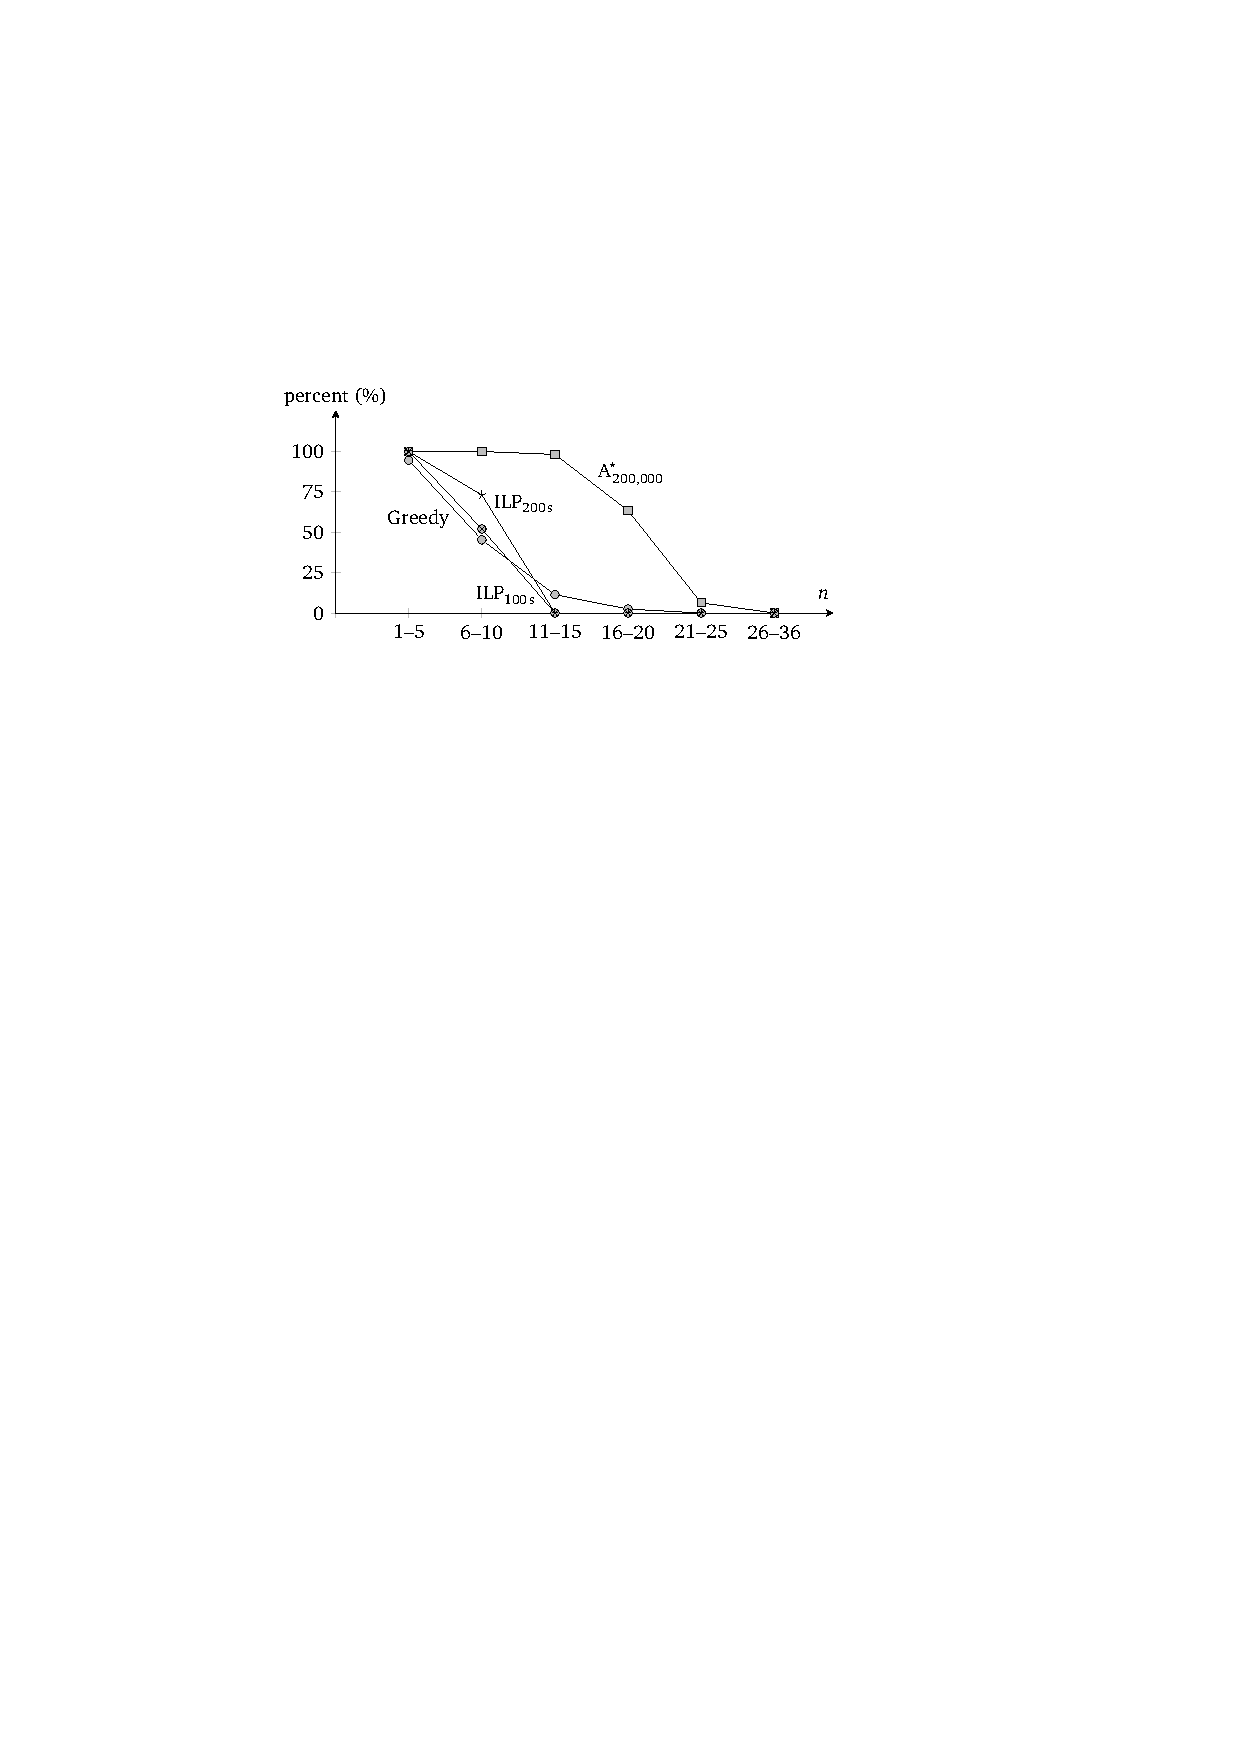
\includegraphics[page=1]{AreaAgg_CaseStudy2_Plot}
\caption{The percentage of regions that were solved 
	optimally by the greedy algorithm, \Astar, and our ILP.
	Note that the numbers of regions according to~$n$ 
	(the number of polygons on the start map in one region) 
	are shown in \fig\ref{fig:AreaAgg_NumRegion}.}
\label{fig:AreaAgg_CaseStudy2_Percentage_Optimal}
%
\par\vspace{\baselineskip} %Leave a gap	between figures
%
\centering
\includegraphics[page=2]{AreaAgg_CaseStudy2_Plot}
\caption{The percentage of regions for which we found at 
	least feasible solutions by the three algorithms.
	Note that the numbers of regions according to~$n$ 
	(the number of polygons on the start map in one region) 
	are shown in \fig\ref{fig:AreaAgg_NumRegion}.}
\label{fig:AreaAgg_CaseStudy2_Percentage_Feasible}
\end{figure}

\begin{figure}[tb]
\centering
\includegraphics[page=3]{AreaAgg_CaseStudy2_Plot}
\caption{The number of regions for which
	our ILP found optimal, feasible, or no solutions 
	when using time limits~$100\,$s and~$200\,$s.
	Using more time, our ILP was able to 
	solve more instances to optimality.}
\label{fig:AreaAgg_CaseStudy2_ILP}
\end{figure}

Among all the instances that were solved to optimality by \Astar
in both experiments (i.e., \sects\ref{sec:AreaAgg_CaseStudy1} 
and~\ref{sec:AreaAgg_CaseStudy2}),
region~$358$ (marked in \tab\ref{tab:CostsInDetail})
is the largest one.
In both experiments, the cost of type change is~$0.044$.
The optimal aggregation sequences for this region
obtained by using costs~$g_1$ and~$g_2$
are shown in \fig\ref{fig:AreaAgg_CaseStudy2_Rg358}.
We, however, noticed some unpleasant aggregates.
The step from~$8$ patches to~$7$ patches 
when using cost function~$g_1$ is a bad move
(see \fig\ref{fig:AreaAgg_CaseStudy2_Rg358}b).
Instead we expect the result of 
\fig\ref{fig:AreaAgg_CaseStudy2_Rg358}a.
Using cost function~$g_2$, we had a similar problem. 
The subdivision with~$7$ patches is such an example,
where we expect the result of 
\fig\ref{fig:AreaAgg_CaseStudy2_Rg358}c.
In an earlier version of this chapter \parencite[see][]{Peng2017AStar},
we tried a combination of minimizing type changes 
and maximizing the sum of the smallest compactness values, 
over the whole sequence.
For that objective, we had a similar problem as 
in \fig\ref{fig:AreaAgg_CaseStudy2_Rg358}b.
This problem, however, can be fixed easily 
by forbidding two patches to aggregate 
if their common boundary is too short.
Moreover, there are two more possible solutions.
First, we could integrate the shared length
into our cost function, as did by \textcite{vanOosterom2005}.
Second, we could weight the cost of shape more heavily
(i.e., increasing weight factor~$\lambda$ of 
\eqs\ref{eq:g_1} and~\ref{eq:g_2}).
According to our experiences, 
the weight factor that we applied defines a reasonable trade-off 
between the different conflicting objectives, 
when considering a solution as a whole. 
However, we are far from claiming that 
the applied weight factor has been optimally chosen. 
This would probably require a user study.

\begin{figure}[h!tb]
\centering
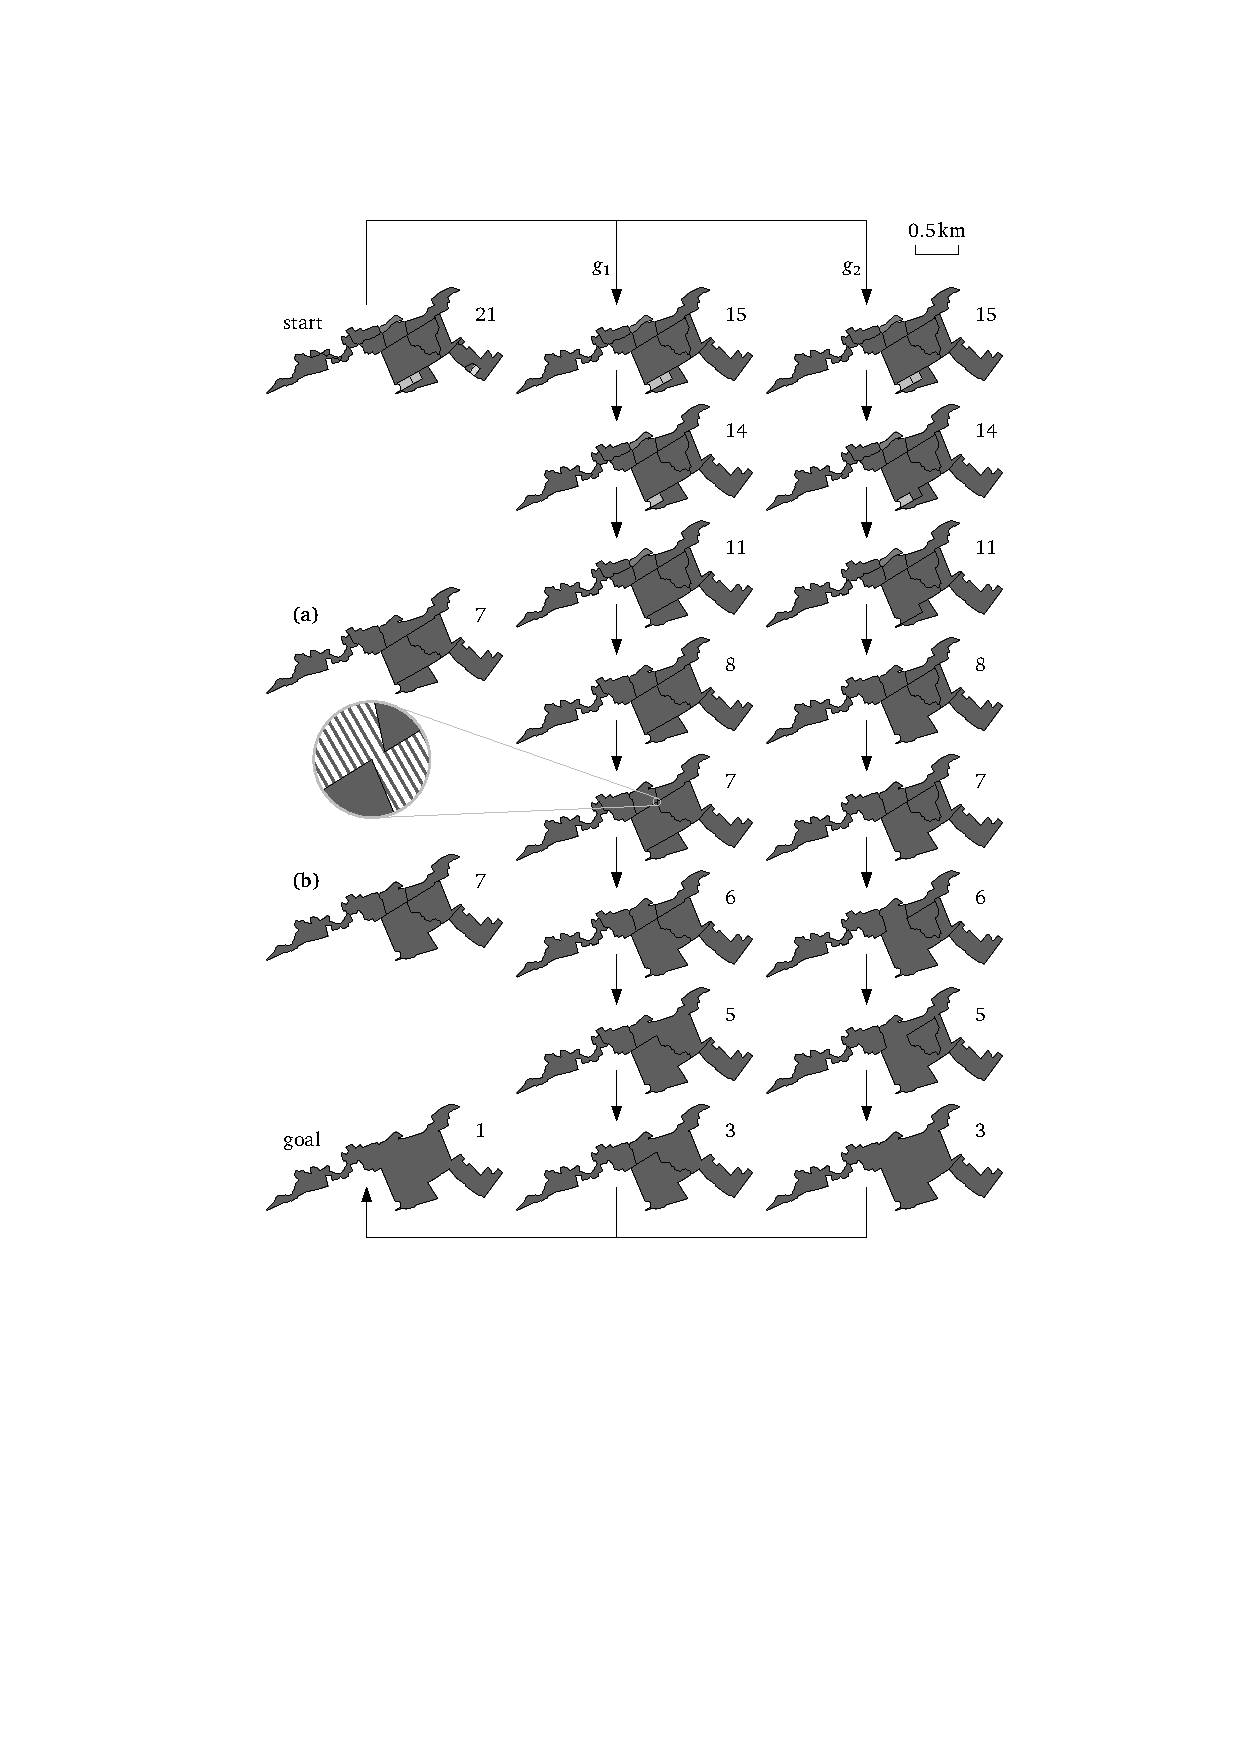
\includegraphics[page=1]{AreaAgg_CaseStudy2}
\caption{Some intermediate subdivisions of region~$358$ 
	obtained by \Astar with different cost functions.
	The numbers indicate the numbers of patches.
    The step from $8$ patches to $7$ patches 
    when using cost function~$g1$ is a bad move; see figure (b). 
    Instead, we expect the result of figure (a). 
    Using cost function~$g2$, we had a similar problem. 
    The subdivision with $7$ patches is such an example, 
    where we expect the result of figure (c).
}
\label{fig:AreaAgg_CaseStudy2_Rg358}
\end{figure}


%\todo{chart: memory use of greedy, A*, and ILP}

\section{Concluding Remarks}
\label{sec:AreaAgg_Conclusions}
In this chapter, we investigated the problem of 
finding optimal sequences for area aggregation.
We compared three methods to solve this problem, namely, 
a greedy algorithm, \Astar, and an ILP-based algorithm.
The greedy algorithm is used as a benchmark.
Unsurprisingly, it ran faster than the other two methods by far.
According to our experiments, \Astar found area aggregation 
sequences
with the least total cost over all regions.
For some instances, however, \Astar had to overestimate
in order to find feasible solutions.
Compared to the greedy algorithm, 
\Astar reduced the total costs by~$2.8\%$ and~$3.9\%$
in the two experiments.
Although the amount is small, it is worth to use \Astar
because optimization methods can help us 
to evaluate the quality of a model 
\parencite{Haunert2017Label,Haunert2008Assuring,Haunert2016Optimization}.
For example, \fig\ref{fig:AreaAgg_CaseStudy2_Rg358}b shows that
even an \emph{optimal} sequence can be bad.
If it were not for \Astar, 
we could not tell if the bad result was caused 
by the greedy algorithm or the model.
Because of \Astar, we are sure that the bad result is from
our model of minimizing the 
type change and the compactness.
The ILP-based algorithm finds optimal solutions for some regions,
but for some of the other regions 
it cannot even find a feasible solution.
Compared to the ILP-based algorithm,
\Astar used less memory 
yet found optimal solutions for more regions.

%\todo[inline]{estimate compactness based on length; cauchy 
%schwarz}

Our \Astar has a good estimation for the cost of type 
change, which helps a lot to reduce the search space. 
Our estimation for the cost of shape 
(compactness or length) is poor.
There are two ways to improve \Astar
in terms of solving more instances to optimality 
while using the same limit of main memory.
First, during the searching we can forget a node of the graph
(see \fig\ref{fig:AreaAgg_SubdivisionName})
if all the neighbors of this node have been visited.
By testing a case, we learned that half of the nodes can be 
forgotten during the pathfinding process.
In this way, we can release some main memory 
and visit more nodes.
Once we arrive at the goal, 
we know the cost for 
an optimal solution (the least cost).
As many visited nodes have been forgotten, 
we do not have the shortest path so far.
We need to run \Astar again.
This time we know for sure that 
a path is not optimal if its cost, 
the sum of the exact cost and the estimated cost, 
is more than the least cost 
(of the optimal solution found previously).
Consequently, we are able to prune some branches earlier 
than the first time we run \Astar.
In this way, we manage to save some main memory.
As a result, we are more likely to find optimal solutions
when the main memory is limited.
Second, if we obtain a solution based on overestimation, 
then we know the cost of this non-optimal solution.
We may decrease the overestimation factor by pruning the branches
that cost more than the non-optimal solution.


We may speed up our ILP-based algorithm using a so-called 
cutting-plane approach as \textcite{Oehrlein2017Aggregation}.
Also, we can add more constraints to
reduce the choices of variables.
For example, assignment to a given center~$r$ is symmetric, 
hence we have
\begin{equation*}
\label{eq:CstrZX}
z_{t,p,q,r}= z_{t,q,p,r} \qquad
\forall t \in {T} \setminus \{1,n\}, 
\forall p, q, r \in P.
\end{equation*}
Whether adding such kinds of constraints always
speeds up our ILP is not clear
because the solver, CPLEX, is a black box to us.
Although integer linear programming may be not good at 
finding optimal sequences for area aggregation,
it is relatively easy to formulate problems as ILPs.
As stated by \citet[p.~861]{Cormen2009}, 
``an efficient algorithm designed specifically for a problem 
will often be more efficient than 
linear programming both in theory and in practice. 
The real power of linear programming comes from 
the ability to solve new problems.''

We may improve both the \Astar algorithm and the ILP-based 
algorithm by integrating the greedy algorithm.
The idea is that we use the greedy algorithm to find 
a solution. 
Then we can use the cost of the solution as an upper bound to 
prune the branches of \Astar and the ILP. 
Once we see that
the cost of a branch is larger than the upper bound,
we can ignore that branch  
because it will not yield an optimal solution.



In cartography, there are many more requirements 
for area aggregation.
For example, one requirement is 
to keep important land-cover areas for a longer time
(such as a settlement surrounded by farmlands).
This requirement can be achieved by incorporating the idea of
\textcite{Dilo2009tGAP}.
They gave each type a weight, 
then defined the importance of a patch 
by the product of the area size and the type weight.
While in our method, we used only the area size as importance.
%
Another requirement is that 
aggregating two areas may result in 
an area with a generalized type,
as did by \textcite{vanSmaalen2003}. 
For example, aggregating 
\emph{farmland} with \emph{hedge} 
yields an area with type \emph{vegetation}.
%
In our setting, we ignored the fact that
some features may inherently take linear forms
(e.g., rivers).
%
These issues can be considered in our future work.
%






